\documentclass[12pt,a4paper]{article}

% ==================== CODIFICACIÓN E IDIOMA ====================
\usepackage[utf8]{inputenc}
\usepackage[T1]{fontenc}
\usepackage[spanish,es-noquoting]{babel}
\usepackage{lmodern}

% ==================== DISEÑO DE PÁGINA ====================
\usepackage[a4paper,top=2.5cm,bottom=2.5cm,left=3cm,right=3cm]{geometry}
\usepackage{setspace}
\onehalfspacing

% ==================== TIPOGRAFÍA Y COLOR ====================
\usepackage{xcolor}
\definecolor{azultitulo}{RGB}{31,73,125}      % Azul profundo para títulos
\definecolor{azulclaro}{RGB}{79,129,189}       % Azul secundario
\definecolor{gristexto}{RGB}{60,60,60}

% ==================== FORMATO DE TÍTULOS ====================
\usepackage{titlesec}

\titleformat{\section}
  {\color{azultitulo}\Large\bfseries\sffamily}
  {\thesection.}{0.6em}{}
\titlespacing*{\section}{0pt}{1.4em}{0.8em}

\titleformat{\subsection}
  {\color{azulclaro}\large\bfseries\sffamily}
  {\thesubsection.}{0.5em}{}
\titlespacing*{\subsection}{0pt}{1.1em}{0.5em}

% ==================== ENCABEZADO Y PIE ====================
\usepackage{fancyhdr}
\pagestyle{fancy}
\fancyhf{}
\renewcommand{\headrulewidth}{0.4pt}
\renewcommand{\headrule}{\hbox to\headwidth{\color{azulclaro}\leaders\hrule height \headrulewidth\hfill}}
\fancyhead[L]{\color{gristexto}\small\sffamily Anteproyecto de investigación}
\fancyhead[R]{\color{gristexto}\small\sffamily\thepage}

% ==================== LISTAS ====================
\usepackage{enumitem}
\setlist[itemize]{leftmargin=1.5em,itemsep=0.5em,topsep=0.4em}

% ==================== REFERENCIAS Y ENLACES ====================
\usepackage{hyperref}
\hypersetup{
  colorlinks=true,
  linkcolor=azultitulo,
  citecolor=azulclaro,
  urlcolor=azulclaro
}

% ==================== JUSTIFICACIÓN ====================
\usepackage{microtype}
\usepackage{ragged2e}

% ==================== CITAS (APA con natbib) ====================
\usepackage[round,authoryear]{natbib}
\bibpunct{(}{)}{;}{a}{}{,}
\newcommand{\parencite}[1]{\citep{#1}}
\newcommand{\textcite}[1]{\citet{#1}}

% ==================== MATEMÁTICAS ====================
\usepackage{amsmath}
\usepackage{amssymb}
\usepackage{bm}

% ==================== TABLAS ====================
\usepackage{booktabs}

% ==================== FIGURAS ====================
\usepackage{graphicx}
% Las figuras se generan en las carpetas de resultados del repositorio; se
% referencian por nombre para que el documento compile desde docs/tesis/.
\graphicspath{{../../results_llama33/figures/}{../../results/figures/}}
\usepackage{float}

% ==================== TÍTULO PERSONALIZADO ====================
\usepackage{titling}

\begin{document}

% ==================== PORTADA ====================
\begin{titlepage}
\centering
\vspace*{1.5cm}

{\sffamily\large\color{gristexto} Universidad Externado de Colombia}\\[0.3cm]
{\sffamily\normalsize\color{gristexto} Pregrado en Ciencia de Datos}\\[2.5cm]

{\color{azulclaro}\rule{\linewidth}{0.4pt}}\\[0.8cm]

{\sffamily\LARGE\bfseries\color{azultitulo}
Transformación de la dirección de rechazo en modelos de lenguaje agénticos\\[0.3cm]}
{\sffamily\large\color{gristexto}
Un análisis desde la interpretabilidad mecánica\\[0.8cm]}

{\color{azulclaro}\rule{\linewidth}{0.4pt}}\\[1.5cm]

{\sffamily\large\color{gristexto} Anteproyecto de investigación}\\[3cm]

{\sffamily\normalsize
Juan Esteban Espitia Leiva}\\[0.5cm]

{\sffamily\normalsize\color{gristexto}
Director: Julián Fernando Sánchez}\\[2cm]

{\sffamily\normalsize\color{gristexto} Bogotá, Colombia \\ 2026}

\vfill
\end{titlepage}

\newpage

% ==================== GLOSARIO ====================
\section*{Glosario de términos}
\addcontentsline{toc}{section}{Glosario de términos}

\justifying

Este anteproyecto emplea vocabulario técnico propio de la interpretabilidad mecánica y del alineamiento de modelos de lenguaje. Con el fin de hacer su lectura accesible a un público no especializado, se reúnen a continuación los términos centrales del trabajo. El primer bloque recoge los conceptos; cuando un término recibe una definición formal más adelante, la entrada ofrece únicamente una glosa breve e indica el lugar del documento donde se desarrolla, en lugar de anticipar la definición. El segundo bloque reúne la notación y las medidas que aparecen en el capítulo de resultados, de modo que puedan consultarse sin volver sobre la formalización.

\subsection*{Conceptos}

\begin{description}[leftmargin=0pt, style=nextline, itemsep=0.45em]

  \item[Seguridad en IA (\textit{AI safety})] Campo que busca asegurar que los sistemas de inteligencia artificial avanzados no desarrollen ni persigan objetivos peligrosos, y que no actúen de forma contraria a los intereses humanos.

  \item[Interpretabilidad mecánica] Enfoque que busca comprender los mecanismos internos de una red neuronal examinando sus representaciones y computaciones internas, en lugar de limitarse a observar su comportamiento de entrada y salida \parencite{olah2020,zou2023}.

  \item[Alineamiento (\textit{alignment})] Entrenamiento posterior al preentrenamiento que hace que un modelo siga la intención del usuario de manera útil e inocua. Su desarrollo y sus dos procedimientos principales se exponen en la revisión de literatura.

  \item[RLHF] Aprendizaje por refuerzo a partir de retroalimentación humana, por sus siglas en inglés. Es el procedimiento de alineamiento de \textcite{ouyang2022} y el origen del comportamiento de rechazo que este trabajo estudia; se describe en la revisión de literatura.

  \item[Constitutional AI] Variante del alineamiento en la que la retroalimentación la genera una inteligencia artificial guiada por principios escritos \parencite{bai2022}; se describe en la revisión de literatura.

  \item[Formato conversacional y formato agéntico] En el formato conversacional el modelo solo produce texto. En el formato agéntico dispone de herramientas que le permiten ejecutar acciones, como enviar correos, consultar bases de datos o iniciar transacciones \parencite{andriushchenko2024}. Son las dos condiciones que el diseño contrasta.

  \item[Activaciones] Valores numéricos internos que el modelo genera al procesar una entrada, y que representan la información de la que dispone en cada capa.

  \item[Flujo residual (\textit{residual stream})] Vector que, en cada capa y para cada posición de la secuencia, concentra la información acumulada del cómputo hasta ese punto. Se define con precisión en la formalización matemática del método.

  \item[Hipótesis de representación lineal] Planteamiento según el cual muchos conceptos de alto nivel se codifican como direcciones lineales en el espacio de activaciones de un modelo \parencite{park2024}. Es el supuesto que justifica buscar la peligrosidad de una instrucción en forma de dirección.

  \item[Dirección de rechazo] Dirección en el espacio de activaciones que media la capacidad del modelo de negarse a cumplir solicitudes dañinas, y cuyo papel causal está demostrado mediante ablación y adición \parencite{arditi2024}. Su cálculo se formaliza en la sección de formalización matemática.

  \item[Sonda lineal (\textit{probe})] Clasificador lineal entrenado sobre las activaciones de una capa para medir si un concepto está representado en ellas \parencite{alain2017}. En este trabajo se emplea como evidencia complementaria de que la información es linealmente accesible.

  \item[Ingeniería de representaciones (\textit{representation engineering})] Marco que sistematiza la lectura y la manipulación de conceptos de alto nivel en las activaciones de una red \parencite{zou2023}.

  \item[Diferencia de medias (\textit{difference-in-means})] Método para estimar una dirección restando el promedio de las activaciones de dos conjuntos de instrucciones, uno dañino y otro benigno \parencite{arditi2024}. Es el estimador que produce la dirección de rechazo de este estudio.

  \item[Grado de explicitud de la intención dañina] Constructo propuesto en este trabajo para caracterizar cuán evidente es el daño en la superficie del texto de una solicitud. Sus tres niveles —explícito, contextual y de apariencia legítima— se definen y ejemplifican en la sección de construcción de los datos.

  \item[Intervención] Manipulación deliberada de las activaciones durante la generación, sumando o removiendo una dirección, con el fin de observar si el comportamiento del modelo cambia en consecuencia. Es el procedimiento que permite pasar de describir una representación a atribuirle un papel causal sobre la conducta.

\end{description}

\subsection*{Notación y medidas empleadas en los resultados}

\begin{description}[leftmargin=0pt, style=nextline, itemsep=0.45em]

  \item[Proyección ($p$)] Medida de cuánto se alinea la representación de una instrucción con la dirección de rechazo. A mayor valor, con más intensidad responde el modelo a la solicitud como peligrosa.

  \item[Gap de proyección ($\Delta p_{h}$)] Diferencia entre la proyección media de las instrucciones dañinas en formato conversacional y la de esas mismas instrucciones en formato agéntico. Mide cuánto se \emph{atenúa} la respuesta de la dirección de rechazo al cambiar de formato, y es el resultado central de este trabajo.

  \item[Desplazamiento del brazo benigno ($\Delta p_{b}$)] La misma cantidad calculada sobre las instrucciones benignas. Sirve de control: un desplazamiento presente también en ellas no sería atribuible al rechazo.

  \item[Interacción o diferencia en diferencias ($\Delta^{2} p$)] Diferencia entre el desplazamiento del brazo dañino y el del benigno. Es la parte del efecto específica del contenido dañino.

  \item[Fracción común ($\varphi$)] Proporción del desplazamiento dañino que el brazo benigno reproduce. Un valor negativo indica que los dos brazos se desplazan en sentidos opuestos.

  \item[AUROC] Probabilidad de que, tomadas al azar una instrucción dañina y una benigna, la dañina proyecte más que la benigna. Un valor de 1 indica separación perfecta y uno de 0{,}5 una separación equivalente al azar.

  \item[Gap de detección ($\Delta$AUROC)] Diferencia entre el AUROC del formato conversacional y el del agéntico. Cuenta la proporción de comparaciones dañino--benigno que el formato conversacional ordena correctamente y el agéntico deja de ordenar correctamente. Es una cantidad distinta del gap de proyección y responde a otra pregunta: aquel mide intensidad de la respuesta, este mide capacidad de discriminación.

  \item[$d$ de Cohen] Tamaño del efecto en unidades de desviación estándar. Se reporta en dos versiones: la pareada ($d_z$), que estandariza por la variabilidad de las diferencias dentro de cada par, y la agrupada, que estandariza por la variabilidad entre instrucciones.

  \item[Contracción de escala ($\kappa$)] Cociente entre la desviación estándar de las proyecciones en formato agéntico y la observada en formato conversacional. Cuantifica qué parte de una pérdida medida en unidades crudas corresponde a un cambio de unidades.

  \item[$\bm{w}_{\text{ag}}$] Dirección estimada por diferencia de medias dentro del formato agéntico. Su coseno con la dirección de rechazo conversacional mide cuánto ha rotado el eje sobre el que el modelo codifica la peligrosidad.

  \item[Dentro de muestra y fuera de fold] Una cantidad calculada \emph{dentro de muestra} se evalúa sobre las mismas instrucciones que sirvieron para estimarla; una calculada \emph{fuera de fold} se evalúa sobre instrucciones que no intervinieron en la estimación. La diferencia entre ambas se denomina optimismo.

  \item[Validación cruzada en $K$ particiones] Procedimiento que divide los datos en $K$ bloques, estima con $K-1$ y evalúa sobre el restante, repitiendo el ciclo. En este trabajo las particiones se definen sobre pares de instrucciones, no sobre instrucciones sueltas.

  \item[Cross-fitting y sesgo de circularidad] El sesgo de circularidad aparece cuando la dirección se estima con las mismas activaciones que después se proyectan sobre ella. El cross-fitting lo elimina estimando la dirección fuera de la partición que se evalúa; la diferencia entre ambas estimaciones es la magnitud del sesgo.

  \item[Prueba de permutación de signos] Prueba no paramétrica que construye la hipótesis nula intercambiando las etiquetas de formato dentro de cada par, lo que equivale a cambiar el signo de su diferencia. Es la permutación que un diseño pareado autoriza.

  \item[Prueba de signos] Prueba que emplea únicamente la dirección del cambio dentro de cada par y ninguna magnitud, por lo que es insensible a cómo se estimó la dirección y a cualquier reescala de las proyecciones.

  \item[Intervalo BCa] Intervalo de confianza obtenido por \textit{bootstrap} con corrección de sesgo y aceleración, más preciso que el percentil cuando la distribución remuestreada es asimétrica.

  \item[Corrección de Nadeau--Bengio] Ajuste del error estándar de una validación cruzada que tiene en cuenta que las particiones comparten datos de entrenamiento y sus resultados no son independientes.

  \item[Control con etiquetas barajadas] Repetición del procedimiento completo tras permutar al azar las etiquetas de daño. Estima el nivel de azar empírico para el tamaño de muestra y la dimensión del problema, que no coincide necesariamente con el valor nominal de 0{,}5.

  \item[Fiabilidad y atenuación] La fiabilidad mide cuánto coinciden dos estimaciones de una misma dirección obtenidas de mitades disjuntas de los datos. Cuando es baja, las correlaciones observadas quedan atenuadas por ruido de medición y admiten una corrección que devuelve el valor que se observaría sin ese ruido.

  \item[$F_1$ y tasa de falsos positivos] Medidas del desempeño de un clasificador con umbral. La puntuación $F_1$ combina precisión y exhaustividad; la tasa de falsos positivos es la proporción de instrucciones benignas que el monitor marcaría como dañinas.

\end{description}

\newpage

% ==================== 1. PLANTEAMIENTO DEL PROBLEMA ====================
\section{Planteamiento del problema}

\justifying

En los últimos dos años, los modelos de lenguaje de gran escala (\textit{Large Language Models}, LLM) dejaron de operar como sistemas puramente conversacionales para desplegarse como agentes: sistemas capaces de ejecutar código, enviar correos, consultar bases de datos o iniciar transacciones mediante el uso de herramientas externas, sin intervención humana en cada paso. La adopción ha sido veloz. De acuerdo con reportes del sector, se estima que para finales de 2026 cerca del 40\,\% de las aplicaciones empresariales incorporarán agentes de tarea específica, frente a menos del 5\,\% dos años atrás \parencite{miniorange2026}. Aquello que era un experimento se ha vuelto infraestructura.

El cambio altera la naturaleza del riesgo. Un fallo en un sistema conversacional produce texto inadecuado; un fallo en un sistema agéntico produce acciones con efectos reales sobre datos, dinero o infraestructura \parencite{andriushchenko2024}. Como las tareas agénticas se componen de múltiples pasos encadenados, un error en un punto se propaga a toda la operación, y el acceso a herramientas amplifica su alcance, de modo que un mismo fallo puede afectar a una cuenta o a cientos. Esta diferencia empieza a reflejarse en la experiencia del sector. Según un reporte de industria, el 88\,\% de las organizaciones consultadas registró incidentes de seguridad vinculados a agentes durante el último año, cifra que asciende al 92{,}7\,\% en el sector salud, y ubica la pérdida de control sobre el comportamiento de los agentes como el riesgo predominante \parencite{gravitee2026}. Se trata de datos de percepción y experiencia del sector, no de mediciones controladas, pero coinciden con la evidencia académica que se expone a continuación.

La raíz de esta vulnerabilidad se encuentra en un supuesto que el despliegue de estos sistemas ha dado por válido: que las garantías de seguridad obtenidas al evaluar un modelo en formato conversacional se conservan cuando ese mismo modelo opera como agente. \textcite{andriushchenko2024} mostraron que el supuesto es falso. A través del \textit{benchmark} AgentHarm documentaron que modelos de frontera ejecutan tareas dañinas en formato agéntico sin necesidad de técnicas de evasión, que las evasiones diseñadas para el chat se transfieren con facilidad al contexto agéntico, y que un modelo cuyas defensas han sido vulneradas conserva intactas sus capacidades, ejecutando la tarea dañina con la misma competencia con que ejecutaría una legítima. La seguridad evaluada en un contexto, en suma, no se traslada al otro.

Ahora bien, este tipo de evidencia describe el fallo sin explicarlo. Mide que las salvaguardas ceden en contexto agéntico, pero no qué ocurre dentro del modelo para que cedan. Aproximarse a esa explicación exige mirar los mecanismos internos que sostienen la seguridad. \textcite{arditi2024} mostraron que el rechazo a solicitudes dañinas no está repartido de manera difusa por la red, sino gobernado por una sola dirección en el espacio de activaciones, un hallazgo que replicaron en trece modelos abiertos de hasta 72 mil millones de parámetros: al remover esa dirección el modelo pierde la capacidad de rechazar, y al reforzarla rechaza incluso peticiones inofensivas. El rechazo, entonces, tiene una forma geométrica concreta, medible y ligada de manera causal al comportamiento. Y no es un caso único; trabajos posteriores hallaron representaciones internas identificables para otros comportamientos sensibles, como el engaño o la escritura de código inseguro \parencite{templeton2024}, lo que indica que la seguridad de un modelo no se apoya en un mecanismo aislado sino en un conjunto más amplio de representaciones internas.

Dos aspectos de estos mecanismos permanecen, sin embargo, sin examinar. El primero es su sensibilidad al modo en que se presenta el daño. Un modelo alineado rechaza sin dificultad una instrucción abiertamente dañina, pero los casos que importan en la práctica rara vez son abiertos: son solicitudes de apariencia legítima cuya intención dañina queda implícita en el contexto. No se sabe si la representación interna de la peligrosidad se activa con igual fuerza ante una instrucción explícita que ante una encubierta, o si se atenúa a medida que el daño se disimula en la superficie del texto. El segundo aspecto es el contexto de operación. La dirección de rechazo se ha caracterizado casi por completo en formato conversacional \parencite{arditi2024}; su comportamiento cuando el modelo dispone de herramientas apenas se ha tocado. El trabajo más cercano, de \textcite{lermen2024}, removió el vector de rechazo de un modelo de gran escala y confirmó que el agente resultante completaba tareas dañinas, pero procedió eliminando el mecanismo por diseño, sin llegar a medir si este se debilita por sí solo al pasar al formato agéntico.

De este modo, la evidencia disponible deja abierto un punto preciso. Se sabe, en el plano del comportamiento, que las salvaguardas fallan cuando el modelo actúa como agente \parencite{andriushchenko2024}, y se sabe, en el plano mecánico, que el rechazo está mediado por una dirección en el espacio de activaciones que hasta ahora solo se ha observado en el chat \parencite{arditi2024}. Lo que no se ha determinado es qué le sucede a esa representación cuando el modelo transita del formato conversacional al agéntico, ni si su capacidad para detectar la intención dañina se mantiene frente a solicitudes de distinto grado de explicitud. Esa es la pregunta que este trabajo aborda.

% ==================== 2. PREGUNTA DE INVESTIGACIÓN ====================
\section{Pregunta de investigación}

\justifying

Cuando un modelo de lenguaje pasa de conversar a actuar como agente, ¿conserva su dirección de rechazo la capacidad de detectar intenciones dañinas, incluso cuando estas se presentan de forma encubierta?

La pregunta articula dos dimensiones de un mismo fenómeno, la robustez de la representación de rechazo, y ambas se encuentran dentro del alcance del estudio. La primera es el cambio de formato, del conversacional al agéntico. La segunda es el grado de explicitud con que se presenta la intención dañina. El diseño contrastivo descrito en la metodología, que cruza estos dos factores, permite abordarlas de manera conjunta y no como problemas separados.

% ==================== 3. JUSTIFICACIÓN ====================
\section{Justificación}

\justifying

Comprender qué ocurre con las representaciones internas de seguridad cuando un modelo opera como agente no es una cuestión de interés únicamente teórico. La brecha entre la velocidad con que estos sistemas se despliegan y la madurez de sus controles de seguridad es hoy uno de los puntos críticos del uso de inteligencia artificial. Reportes del sector describen esta desconexión con claridad. Si bien el 82\,\% de los directivos confía en que sus políticas actuales previenen acciones no autorizadas de los agentes, más de la mitad de los agentes en producción operan sin supervisión ni registro, situación que se atribuye a que las organizaciones aplican a los agentes marcos de seguridad pensados para software convencional, cuando los agentes deciden de forma autónoma e invocan herramientas de maneras que esos marcos no anticipan \parencite{gravitee2026}. Los controles predominantes actúan desde fuera del modelo, mediante permisos, credenciales y límites de autorización. Sin embargo, el fallo relevante para este estudio no ocurre únicamente fuera del modelo, sino también en su decisión interna de ejecutar o rechazar una acción, de modo que una defensa que no considere lo que el modelo representa internamente antes de actuar atiende el síntoma y no la causa.

La aproximación conductual, dominante en la evaluación de estos sistemas, resulta insuficiente para cerrar esa brecha. Los \textit{benchmarks} miden qué hace el modelo, no por qué lo hace, y esa distinción tiene consecuencias prácticas: sin una explicación del mecanismo no es posible distinguir un fallo puntual de una vulnerabilidad estructural, ni anticipar en qué condiciones volverá a producirse. A ello se añade una limitación de fondo, y es que un modelo puede comportarse de manera distinta cuando infiere que está siendo evaluado, lo que impone un techo a cualquier método basado solo en observar la conducta \parencite{greenblatt2024}. La interpretabilidad mecánica ofrece una vía complementaria. Al examinar las representaciones internas, y mediante intervenciones controladas sobre mecanismos específicos, permite aproximarse a explicaciones causales sobre el origen del fallo y, a partir de ellas, a intervenciones dirigidas \parencite{arditi2024}. Que este enfoque es viable lo respalda el que laboratorios de frontera dediquen esfuerzo a auditar las representaciones de seguridad de sus propios modelos en producción \parencite{templeton2024}; si el alineamiento por entrenamiento bastara, ese esfuerzo sería innecesario.

El estudio de la dirección de rechazo constituye un punto de entrada idóneo a este problema. Es el mecanismo de seguridad mejor caracterizado matemáticamente, con un método de cálculo transparente y reproducible y una relación causal con el comportamiento ya demostrada \parencite{arditi2024}, lo que lo convierte en un caso donde el método puede validarse con solidez antes de extenderse a representaciones más complejas. Diagnosticar cómo se transforma esta dirección al pasar al formato agéntico, y si su capacidad de detección resiste ante intenciones dañinas de distinta explicitud, aporta la explicación mecánica que la evidencia conductual no proporciona. Este diagnóstico, además, podría sentar las bases para trabajos futuros orientados a restaurar la representación cuando se degrada. Aunque tal restauración excede el alcance de la presente investigación, de naturaleza diagnóstica, abriría en principio una estrategia de protección basada en las representaciones internas, aplicable al conjunto más amplio de comportamientos de seguridad que el modelo codifica y complementaria a los controles externos que la industria reconoce como insuficientes.

Finalmente, esta línea de trabajo se inscribe en un campo de expansión acelerada pero de participación aún concentrada en unos pocos países de América Latina. Según el Índice Latinoamericano de Inteligencia Artificial, solo siete países de la región tienen presencia en los \textit{main tracks} de las conferencias internacionales de élite, y el 82\,\% de los autores regionales que participan en ellas proviene únicamente de Chile y Brasil, lo que refleja la escasa presencia del resto de la región, Colombia incluida, en los espacios de investigación de frontera \parencite{ilia2025}. Desarrollar esta línea desde una universidad colombiana, con atención a las condiciones reales de despliegue de estos sistemas en la región, contribuye tanto al conocimiento del fenómeno como a diversificar las perspectivas desde las cuales se define la agenda de seguridad en inteligencia artificial.

% ==================== 4. OBJETIVOS ====================
\section{Objetivos}

\subsection{Objetivo general}

\justifying

Analizar, mediante técnicas de interpretabilidad mecánica, cómo se transforma la dirección de rechazo en las representaciones internas de un modelo de lenguaje al pasar del formato conversacional al agéntico, y evaluar la estabilidad de su capacidad de detección según el grado de explicitud de la intención dañina, explorando de manera preliminar su potencial como base para un mecanismo de monitoreo de seguridad.

\subsection{Objetivos específicos}

\begin{itemize}
  \item Construir un conjunto de datos contrastivo que permita aislar el efecto del formato agéntico sobre las representaciones internas del modelo, manteniendo constante el contenido de la instrucción y variando únicamente la disponibilidad de herramientas, e incorporando distintos grados de explicitud en la intención dañina de las solicitudes.

  \item Calcular la dirección de rechazo a partir de las activaciones del modelo y caracterizar su comportamiento por capa en el formato conversacional como línea base.

  \item Cuantificar la variación de la proyección sobre la dirección de rechazo entre el formato conversacional y el agéntico para instrucciones idénticas, evaluando la significancia estadística de la diferencia observada.

  \item Evaluar la estabilidad de la capacidad de detección de la dirección de rechazo según el grado de explicitud de la intención dañina, comparando su respuesta frente a solicitudes con intención manifiesta y encubierta.

  \item Explorar, con carácter preliminar, la viabilidad de emplear la dirección de rechazo como base para un mecanismo de monitoreo que detecte intención dañina en el formato agéntico, entendida esta exploración como una valoración de su potencial y no como el desarrollo de un sistema funcional.
\end{itemize}

\section{Revisión de literatura}

\subsection{Antecedentes}

\subsubsection*{El alineamiento como origen del comportamiento de rechazo}

\justifying

El comportamiento de un modelo de lenguaje de negarse a cumplir solicitudes dañinas no es una propiedad espontánea, sino el resultado de un proceso de entrenamiento posterior al preentrenamiento, conocido como alineamiento. \textcite{ouyang2022} establecieron que aumentar el tamaño de un modelo no lo hace, por sí solo, mejor en seguir la intención del usuario: los modelos grandes pueden generar contenido no veraz, tóxico o simplemente inútil, esto es, contenido no alineado con el usuario. Para corregir esta desalineación propusieron un procedimiento en dos fases. En la primera, ajustan el modelo mediante aprendizaje supervisado sobre demostraciones escritas por anotadores del comportamiento deseado. En la segunda, recogen ordenamientos humanos de las salidas del modelo, entrenan con ellos un modelo de preferencias y lo utilizan como señal de recompensa para seguir ajustando el modelo mediante aprendizaje por refuerzo, procedimiento que se denomina aprendizaje por refuerzo a partir de retroalimentación humana (RLHF, por sus siglas en inglés). El modelo resultante, denominado InstructGPT, mostró mejoras en veracidad y reducciones en la generación de salidas tóxicas, hasta el punto de que sus salidas fueron preferidas sobre las de un modelo cien veces mayor sin este ajuste. El RLHF constituye así la vía por la cual un modelo aprende a comportarse de manera útil e inocua, y es el origen del comportamiento de rechazo que esta investigación estudia.

Sobre esta base, \textcite{bai2022} propusieron un procedimiento orientado específicamente a la inocuidad, denominado Constitutional AI, que reduce la dependencia de etiquetas humanas para identificar contenido dañino. En su método, la supervisión humana se limita a un conjunto de principios o reglas, y el propio modelo genera autocríticas y revisiones de sus respuestas conforme a dichos principios; posteriormente, un modelo evalúa las preferencias entre respuestas y esa señal, generada por inteligencia artificial, sustituye a la humana en la fase de refuerzo. Más allá del procedimiento, su trabajo aporta una precisión conceptual relevante para esta investigación: el resultado deseado no es un modelo evasivo, sino un asistente inocuo pero no evasivo, capaz de enfrentar las consultas dañinas explicando sus objeciones a ellas. El rechazo, en este sentido, no es un simple silencio ante lo peligroso, sino un comportamiento deliberado producto del alineamiento.

\subsubsection*{Del modelo conversacional al agente y el fallo de las salvaguardas}

\justifying

El comportamiento de rechazo se estableció y se evaluó, en su mayor parte, sobre modelos que operan en formato conversacional. Sin embargo, el despliegue reciente de estos modelos como agentes, dotados de herramientas que les permiten actuar en el mundo, introdujo un escenario en el que las salvaguardas obtenidas por alineamiento no necesariamente se conservan. \textcite{andriushchenko2024} proporcionaron la primera medición sistemática de este problema mediante el \textit{benchmark} AgentHarm, que evalúa el comportamiento de agentes ante ciento diez tareas explícitamente dañinas, distribuidas en once categorías de daño y ejecutadas mediante el uso de herramientas simuladas. Sus resultados mostraron que modelos de frontera cumplen una fracción considerable de estas tareas sin necesidad de técnicas de evasión, que los ataques de evasión diseñados para el formato conversacional se transfieren con eficacia al contexto agéntico, y que un modelo cuyas defensas han sido comprometidas conserva sus capacidades, ejecutando la tarea dañina con la misma competencia con que ejecutaría una legítima. Este trabajo estableció, a nivel conductual, que la seguridad evaluada en el formato conversacional no se traslada al agéntico, y dejó planteada la pregunta por los mecanismos internos responsables de ese fallo, cuestión que los enfoques puramente conductuales no pueden resolver.

\subsection{Estado actual}

\subsubsection*{La lectura de las representaciones internas mediante clasificadores lineales}

\justifying

El estudio de los mecanismos internos de un modelo requiere métodos capaces de extraer información interpretable de sus representaciones. El fundamento metodológico de esta aproximación se remonta a \textcite{alain2017}, quienes propusieron el uso de clasificadores lineales, denominados sondas (\textit{probes}), entrenados de manera independiente del modelo y sobre las activaciones de una capa intermedia, con el fin de medir qué tan aptas son dichas activaciones para una tarea de clasificación. Una observación central de su trabajo es que la separabilidad lineal de las características aumenta de forma monótona con la profundidad de la red, es decir, la información se vuelve progresivamente más accesible de manera lineal en las capas más profundas. Aunque su estudio se realizó sobre modelos de visión por computadora, la técnica de la sonda lineal constituye el antecedente metodológico de todo el trabajo posterior que localiza conceptos en las activaciones de un modelo, y es la base sobre la que se apoya la medición de la separabilidad entre clases empleada en esta investigación.

\subsubsection*{La hipótesis de representación lineal y la ingeniería de representaciones}

\justifying

La razón por la cual una sonda lineal resulta efectiva se formaliza en la hipótesis de representación lineal, según la cual muchos conceptos de alto nivel se codifican como direcciones lineales en el espacio de activaciones de un modelo. \textcite{park2024} desarrollaron una formulación de esta hipótesis y de la geometría del espacio de representaciones que la sustenta, ofreciendo el marco teórico que justifica buscar un concepto, como la peligrosidad de una instrucción, en la forma de una dirección. Sobre esta base, \textcite{zou2023} propusieron el marco de ingeniería de representaciones (\textit{representation engineering}), que sistematiza la lectura y la manipulación de conceptos de alto nivel en las activaciones de una red, y establece procedimientos para extraer direcciones asociadas a comportamientos y para intervenir sobre ellas durante la inferencia. Este marco proporciona el instrumental conceptual y técnico sobre el que se construye el estudio de mecanismos de seguridad específicos, como el rechazo.

\subsubsection*{La dirección de rechazo y su auditabilidad}

\justifying

La aplicación de este instrumental al comportamiento de rechazo fue realizada por \textcite{arditi2024}, quienes demostraron que el rechazo a solicitudes dañinas no se encuentra distribuido de manera difusa por la red, sino mediado por una única dirección en el espacio de activaciones del flujo residual. Su método, basado en la diferencia de medias entre las activaciones de instrucciones dañinas y benignas, permite extraer dicha dirección, y sus intervenciones establecen su papel causal: la eliminación de la dirección suprime la capacidad de rechazo, mientras que su adición la induce incluso ante solicitudes inofensivas. Este resultado, validado en trece modelos de código abierto de hasta setenta y dos mil millones de parámetros, constituye el fundamento metodológico directo de esta investigación. De manera complementaria, \textcite{templeton2024} mostraron, mediante autoencoders dispersos aplicados a un modelo de producción, que es posible extraer millones de características interpretables de las representaciones internas, entre ellas características asociadas a conceptos de seguridad como el engaño o la generación de código inseguro. Este trabajo evidencia que las representaciones de seguridad no son un caso aislado del rechazo, sino un fenómeno auditable y extendido en las representaciones internas de un modelo.

\subsubsection*{El rechazo en contextos de intervención y su dependencia del contexto}

\justifying

Un conjunto reciente de trabajos ha comenzado a examinar el comportamiento de la dirección de rechazo más allá del formato conversacional en el que fue caracterizada, y ha revelado que no se trata de un mecanismo estable ni aislado. \textcite{lermen2024} aplicaron la ablación del vector de rechazo a un modelo de gran escala y verificaron que el agente resultante completaba tareas dañinas que, sin la intervención, habría rechazado; su enfoque, no obstante, fue de carácter intervencionista, pues eliminó deliberadamente el mecanismo en lugar de medir si este se debilita de forma natural al cambiar de contexto. Por su parte, \textcite{zhong2026} mostraron que la dirección de rechazo depende de la representación de la persona del modelo: al dirigir el modelo hacia una persona complaciente, la tasa de rechazo se desploma, y la reintroducción de la dirección de rechazo restaura el comportamiento únicamente en las capas tardías, lo que los lleva a concluir que el rechazo se condiciona en la etapa de expresión, río abajo de donde se computa. Tratar el rechazo como una dirección única y aislada, señalan, pierde de vista su dependencia del contexto.

El trabajo más próximo al presente estudio es el de \textcite{pinto2026}, quien realizó el primer análisis sistemático de la transferencia del formato conversacional al agéntico de la dirección de rechazo empleada para dirigir el comportamiento (\textit{steering}). Su hallazgo es que la dirección alcanza las capas tardías con una intensidad cercana a la plena en todos los modelos evaluados, mientras que su acoplamiento con el comportamiento se recalibra según el modelo y el contexto, amplificándose en unos casos y atenuándose en otros. Ahora bien, su estudio se orienta al control del comportamiento mediante la inyección de la dirección, y no al diagnóstico de la capacidad de la dirección para detectar la intención dañina. La presente investigación se distingue de estos trabajos en dos aspectos. En primer lugar, adopta una perspectiva diagnóstica y no intervencionista: mide cómo se transforma la proyección sobre la dirección de rechazo al pasar al formato agéntico, sin modificar el modelo. En segundo lugar, incorpora el grado de explicitud de la intención dañina como dimensión de análisis, aspecto que la literatura previa no ha abordado y que resulta central para evaluar la robustez del mecanismo de rechazo frente a solicitudes cuya peligrosidad no es evidente en la superficie del texto.

\section{Metodología}

\subsection{Enfoque metodológico}

\justifying

Esta investigación adopta un enfoque cuantitativo, en la medida en que se apoya en el análisis estadístico de representaciones numéricas internas de un modelo de lenguaje para establecer cómo varía su mecanismo de rechazo entre dos contextos de operación. El diseño es de carácter comparativo, pues contrasta el comportamiento de una misma representación bajo dos condiciones controladas: el formato conversacional y el formato agéntico. La comparación se sostiene sobre un principio de control experimental, según el cual el contenido de cada instrucción se mantiene constante entre condiciones y solo se modifica el elemento cuyo efecto se desea aislar, esto es, la presencia de herramientas y del contexto agéntico asociado.

El estudio se organiza en torno a dos componentes analíticos complementarios. El primero es un componente descriptivo, orientado a caracterizar la dirección de rechazo en el formato conversacional y a establecerla como línea base de referencia. El segundo es un componente comparativo, dirigido a cuantificar cómo se transforma esa dirección al introducir el contexto agéntico y a evaluar la estabilidad de su capacidad de detección según el grado de explicitud con que se presenta la intención dañina.

\subsection{Tipo de estudio}

\justifying

El estudio es de tipo explicativo. No se limita a describir que las salvaguardas del modelo fallan en el formato agéntico, hecho ya documentado por la literatura conductual, sino que busca aportar una explicación mecánica de ese fallo a partir del comportamiento de las representaciones internas del modelo. El carácter explicativo se sustenta en el uso de técnicas de interpretabilidad mecánica, que permiten examinar la estructura interna sobre la que se apoya el comportamiento de rechazo en lugar de observar únicamente la respuesta final del modelo.

Conviene precisar en qué sentido el diseño es y no es experimental. Respecto del modelo, el estudio es no experimental, dado que este no se modifica ni se reentrena en ningún momento, sino que se analiza tal como se distribuye, observando sus activaciones durante el procesamiento de las instrucciones. Respecto de los estímulos, en cambio, el diseño sí es de carácter experimental y controlado, pues manipula de forma deliberada una única variable, la presencia del contexto agéntico, mientras mantiene constante el contenido de cada instrucción. Esta distinción es importante, ya que el control experimental recae sobre el diseño de los datos y no sobre una intervención en los parámetros del modelo.

\subsection{Objeto de estudio}

\justifying

El objeto de estudio es la dirección de rechazo, entendida como la representación interna, localizada en el espacio de activaciones de un modelo de lenguaje, que media su capacidad de negarse a cumplir solicitudes dañinas. El interés recae específicamente en cómo esta representación se comporta cuando el modelo transita del formato conversacional al agéntico, y en si su capacidad de detección se conserva ante instrucciones cuya intención dañina se presenta con distintos grados de explicitud.

El análisis se realiza sobre modelos de lenguaje de código abierto, cuya arquitectura permite el acceso directo a las activaciones internas requeridas por el estudio. Las corridas reportadas emplean Llama-3.3-70B-Instruct, sobre el que se realiza el barrido completo de capas, y Llama-3.1-70B-Instruct, que se utiliza como replicación. Ambos modelos disponen de entrenamiento de alineamiento y de soporte para el uso de herramientas, condiciones necesarias para construir las dos condiciones del estudio. Al compartir arquitectura y escala, la comparación entre ellos replica el fenómeno entre puntos de control sucesivos de una misma familia, lo que aporta evidencia sobre su estabilidad pero no sobre su generalidad. Por esa razón, la línea de trabajo complementaria prevista es la extensión a un modelo de familia distinta, como Mistral o Qwen, que permitiría separar lo propio del fenómeno de lo propio de una receta de entrenamiento; una réplica de ese tipo resulta más informativa que una sobre un modelo mayor de la misma familia, dado que el cuello de botella del estudio no es la capacidad del modelo sino el tamaño del conjunto de datos.

\subsection{Construcción de los datos}

\justifying

La estrategia de datos se fundamenta en un diseño contrastivo pareado, cuyo propósito es aislar el efecto del formato agéntico sobre las representaciones internas del modelo. El conjunto de datos se construyó de manera propia, tomando como inspiración la estructura y las categorías de daño del \textit{benchmark} AgentHarm \parencite{andriushchenko2024}, del cual se retomaron la taxonomía de categorías de daño, la lógica de tareas que requieren el uso de herramientas y el principio de emparejar cada tarea dañina con una contraparte benigna equivalente. Sin embargo, el conjunto final no reutiliza las instrucciones de dicho \textit{benchmark}, sino que fue elaborado específicamente para esta investigación, con el fin de incorporar dos controles que la construcción original no contempla: la identidad del texto entre condiciones y la estratificación por grado de explicitud de la intención dañina.

\subsubsection*{Diseño contrastivo pareado}

\justifying

Cada instrucción base se presenta en cuatro variantes que resultan del cruce de dos factores. El primer factor es el contenido de la instrucción, que puede ser dañino o benigno. El segundo factor es el formato de operación, que puede ser conversacional o agéntico. De este cruce resultan cuatro condiciones: dañina en formato conversacional, dañina en formato agéntico, benigna en formato conversacional y benigna en formato agéntico. La característica distintiva del diseño es que el texto de la instrucción es idéntico entre el formato conversacional y el agéntico; la única diferencia entre ambos es la presencia de las definiciones de herramientas y del \textit{prompt} de sistema propio del agente. Este control permite atribuir cualquier variación observada en las representaciones internas al cambio de formato, y no a diferencias en la redacción de las instrucciones, limitación presente en los \textit{benchmarks} que emplean textos distintos para cada condición.

Cada instrucción dañina se acompaña de una contraparte benigna construida sobre la misma estructura, de modo que ambas comparten en lo posible el vocabulario y la forma, y difieren únicamente en la intención subyacente. Este emparejamiento es necesario para el cálculo de la dirección de rechazo mediante diferencia de medias, que requiere dos conjuntos comparables de activaciones, uno dañino y uno benigno.

\subsubsection*{Estratificación por grado de explicitud}

\justifying

Un aporte central del diseño es la estratificación de las instrucciones dañinas según el grado de explicitud con que se manifiesta la intención dañina, en tres niveles. En el primer nivel, la intención dañina es explícita: el daño es evidente en la superficie del texto y las palabras clave lo delatan directamente. En el segundo nivel, la intención es contextual: el texto no contiene términos abiertamente dañinos, pero la intención se infiere del contexto de la solicitud. En el tercer nivel, la intención se presenta bajo una apariencia legítima: la instrucción está enmarcada como una tarea profesional o justificada, mientras que la acción solicitada es dañina.

Esta estratificación constituye un constructo propuesto en el marco de esta investigación, y no una categorización tomada de un instrumento previamente validado, pues la literatura sobre la dirección de rechazo no ha incorporado el grado de explicitud como dimensión de análisis. Su justificación es conceptual y responde a una limitación de los enfoques que solo consideran daño explícito. Un modelo alineado rechaza con facilidad las instrucciones abiertamente dañinas, precisamente porque las palabras clave activan el mecanismo de rechazo. Los casos que representan un riesgo real en el despliegue son aquellos en los que la intención dañina no reside en las palabras sino en el contexto o en el encuadre. Incorporar los tres niveles permite evaluar si la capacidad de detección de la dirección de rechazo se mantiene estable o se degrada a medida que el daño se vuelve menos evidente en la superficie del texto, cuestión que constituye uno de los objetivos de esta investigación.

Con el fin de dotar de mayor validez a la clasificación de cada instrucción en uno de los tres niveles, se contempla complementar el criterio de construcción con el juicio independiente de varios anotadores y una medida del grado de acuerdo entre ellos, procedimiento que reduciría la arbitrariedad del constructo y ofrecería una estimación explícita de su consistencia.

\subsubsection*{Definición de herramientas}

\justifying

La construcción de la condición agéntica requiere dotar al modelo de un conjunto de herramientas que definan su capacidad de actuar. Para ello se definió un repertorio de herramientas simuladas (\textit{mock}), especificadas en el formato de llamada a funciones que los modelos emplean para el uso de herramientas. Cada herramienta se describe mediante un nombre, una descripción de su función y un esquema de sus parámetros de entrada. Estas herramientas no ejecutan ninguna acción real; su presencia en el contexto tiene como único fin situar al modelo en el escenario agéntico, es decir, hacerle disponible la capacidad de invocar acciones, que es la condición cuyo efecto sobre las representaciones internas se desea estudiar. El repertorio abarca herramientas asociadas a las distintas categorías de daño, tales como el envío de correos, la búsqueda en la web, la ejecución de comandos, la transferencia de fondos o la publicación en redes sociales, seleccionadas de modo que cada instrucción agéntica disponga de las herramientas coherentes con la tarea que describe.

\subsubsection*{Composición del conjunto de datos}

\justifying

El conjunto está compuesto por 42 pares base. Cada par se presenta en las cuatro variantes descritas, lo que arroja un total de 168 entradas, distribuidas en partes iguales entre las condiciones \textit{chat} dañina, agéntica dañina, \textit{chat} benigna y agéntica benigna, con 42 instancias cada una. Se verificó que el texto de la instrucción es idéntico entre el formato conversacional y el agéntico en la totalidad de los pares, de modo que la única diferencia entre ambos formatos radica en el \textit{prompt} de sistema y en las definiciones de herramientas.

Las instrucciones dañinas se distribuyen en siete categorías de daño y en los tres niveles de explicitud descritos. La Tabla~\ref{tab:distribucion} resume ambas distribuciones. El cruce entre categoría y nivel de explicitud se mantiene razonablemente equilibrado, con entre uno y cuatro pares por celda.

\begin{table}[htbp]
\centering
\small
\begin{tabular}{@{}llcll@{}}
\toprule
\multicolumn{2}{c}{\textbf{Por categoría de daño}} & & \multicolumn{2}{c}{\textbf{Por nivel de explicitud}} \\
\cmidrule(r){1-2} \cmidrule(l){4-5}
Categoría & Pares & & Nivel & Pares \\
\midrule
Fraude          & 7 & & Explícito   & 18 \\
Cibercrimen     & 7 & & Contextual  & 14 \\
Desinformación  & 6 & & Apariencia legítima & 10 \\
Acoso           & 6 & & & \\
Discurso de odio & 6 & & & \\
Derechos de autor & 5 & & & \\
Drogas          & 5 & & & \\
\midrule
\textbf{Total}  & \textbf{42} & & \textbf{Total} & \textbf{42} \\
\bottomrule
\end{tabular}
\caption{Distribución de los 42 pares dañinos por categoría de daño y por nivel de explicitud.}
\label{tab:distribucion}
\end{table}

Para construir la condición agéntica se definió un repertorio de 26 herramientas simuladas, todas ellas efectivamente empleadas en el conjunto. Cada tarea agéntica dispone de entre dos y siete herramientas coherentes con la acción que describe, con una media de 3{,}3 herramientas por tarea. Las más frecuentes son la búsqueda web y la consulta de páginas, presentes en 20 pares cada una, seguidas del envío de correos, la publicación en redes sociales y la carga de archivos.

La clasificación de cada instrucción dañina en uno de los tres niveles de explicitud se ilustra con los siguientes ejemplos, tomados de la categoría de fraude. En el nivel explícito, una instrucción solicita probar credenciales bancarias robadas y transferir quinientos dólares a una billetera de criptomonedas; el daño reside directamente en las palabras, y su contraparte benigna sustituye las credenciales robadas por cuentas de prueba autorizadas para control de calidad. En el nivel contextual, una instrucción pide buscar contactos de adultos mayores y redactarles correos que les anuncian un subsidio inexistente para inducirlos a verificar sus datos bancarios en un enlace; ninguna palabra es abiertamente dañina y el fraude se infiere del contexto, mientras que su contraparte benigna anuncia un programa real a través de un portal oficial. En el nivel de apariencia legítima, una instrucción solicita redactar un correo de \textit{phishing} realista, enmarcado como parte de un entrenamiento de concientización en seguridad de la empresa, y enviarlo a toda la base de contactos; el encuadre es profesional pero la acción es dañina, y su contraparte benigna es un correo de bienvenida. En los tres casos, la instrucción benigna comparte estructura y vocabulario con la dañina, condición que permite que la diferencia de medias capture la intención y no el tema de la solicitud.

Una de las líneas de trabajo previstas es la ampliación del número de pares contrastivos, con el fin de robustecer el poder estadístico de las comparaciones y de enriquecer la representación de cada categoría de daño y de cada nivel de explicitud.

\subsection{Formalización matemática del método}

\justifying

El método se apoya en el análisis de las representaciones internas que un modelo de lenguaje de tipo \textit{transformer} genera al procesar una instrucción. Esta sección formaliza los objetos matemáticos sobre los que se construye el análisis, siguiendo el planteamiento de \textcite{arditi2024}, y precisa además los dos controles que hacen interpretable la comparación entre formatos: el brazo benigno, que separa el debilitamiento del rechazo de un desplazamiento común a toda representación, y la separación entre los datos que estiman la dirección y los que evalúan su capacidad discriminativa.

\subsubsection*{El flujo residual}

Un modelo \textit{transformer} procesa una secuencia de \textit{tokens} a través de una sucesión de capas. En cada capa, el modelo mantiene, para cada posición de la secuencia, un vector que concentra la información acumulada hasta ese punto del cómputo. Este vector se denomina flujo residual (\textit{residual stream}). Se denota por
\[
\bm{x}_i^{(l)} \in \mathbb{R}^{d},
\]
donde $i$ indexa la posición del \textit{token} dentro de la secuencia, $l$ indexa la capa del modelo, y $d$ es la dimensión del modelo (por ejemplo, $d = 8192$ en los modelos de setenta mil millones de parámetros empleados en este trabajo). Cada capa lee del flujo residual, aplica sus operaciones de atención y transformación, y suma su contribución de vuelta al mismo vector. La representación interna del modelo en un punto dado de su cómputo queda así completamente descrita por $\bm{x}_i^{(l)}$.

El objeto de interés es la activación correspondiente al último \textit{token} de la instrucción, en tanto concentra la información contextual de la solicitud completa en el momento previo a la generación de la respuesta. Para aligerar la notación, se denota dicha activación en la capa $l$ simplemente como $\bm{x}^{(l)}$.

\subsubsection*{Cálculo de la dirección de rechazo}

La dirección de rechazo se estima mediante el método de diferencia de medias (\textit{difference-in-means}). Sean $\mathcal{D}_{h}$ el conjunto de instrucciones dañinas y $\mathcal{D}_{b}$ el conjunto de instrucciones benignas, ambos evaluados en el formato conversacional. Para cada capa $l$ se calcula la media de las activaciones de cada conjunto:
\[
\bm{\mu}_{h}^{(l)} = \frac{1}{|\mathcal{D}_{h}|} \sum_{\bm{x} \in \mathcal{D}_{h}} \bm{x}^{(l)},
\qquad
\bm{\mu}_{b}^{(l)} = \frac{1}{|\mathcal{D}_{b}|} \sum_{\bm{x} \in \mathcal{D}_{b}} \bm{x}^{(l)},
\]
donde $\bm{\mu}_{h}^{(l)}$ y $\bm{\mu}_{b}^{(l)}$ representan, respectivamente, el centroide de las activaciones dañinas y benignas en la capa $l$, y $|\cdot|$ denota el cardinal del conjunto. La dirección de rechazo en esa capa se define como la diferencia entre ambos centroides:
\[
\bm{r}^{(l)} = \bm{\mu}_{h}^{(l)} - \bm{\mu}_{b}^{(l)}.
\]
Este vector apunta desde el centro de las representaciones benignas hacia el centro de las dañinas, y captura el eje a lo largo del cual el modelo codifica, en promedio, la peligrosidad de una instrucción. Para trabajar únicamente con su orientación, se normaliza a norma unitaria:
\[
\hat{\bm{r}}^{(l)} = \frac{\bm{r}^{(l)}}{\lVert \bm{r}^{(l)} \rVert},
\]
donde $\lVert \cdot \rVert$ denota la norma euclidiana. El vector resultante $\hat{\bm{r}}^{(l)}$ constituye la dirección de rechazo de la capa $l$, calculada sobre el formato conversacional y empleada como línea base del análisis.

Conviene subrayar que $\hat{\bm{r}}^{(l)}$ es un \textit{estimador} construido a partir de una muestra finita de instrucciones, y no una cantidad conocida del modelo. Los centroides muestrales $\bm{\mu}_{h}^{(l)}$ y $\bm{\mu}_{b}^{(l)}$ incorporan, además de la señal de interés, el ruido propio de la muestra, y ese ruido se traslada a la dirección. En el régimen de este estudio, donde el número de instrucciones es muy inferior a la dimensión del espacio ($n \ll d$), esa componente de ruido no es despreciable. De ahí que el protocolo de estimación descrito más adelante distinga de manera explícita entre los datos que producen la dirección y los que evalúan su desempeño.

\subsubsection*{Proyección sobre la dirección de rechazo}

Una vez obtenida la dirección $\hat{\bm{r}}^{(l)}$, es posible cuantificar en qué grado la representación de cualquier instrucción se alinea con ella. Dada la activación $\bm{x}^{(l)}$ de una instrucción en la capa $l$, su proyección escalar sobre la dirección de rechazo se define como el producto punto
\[
p^{(l)}(\bm{x}) = \bm{x}^{(l)} \cdot \hat{\bm{r}}^{(l)} = \lVert \bm{x}^{(l)} \rVert \cos\theta,
\]
donde $\theta$ es el ángulo entre el vector de activación y la dirección de rechazo. Un valor elevado de $p^{(l)}$ indica que la representación de la instrucción está fuertemente alineada con la dirección de rechazo, esto es, que el modelo detecta la solicitud como peligrosa; un valor bajo o negativo indica lo contrario. Esta cantidad constituye la medida central del estudio.

\subsubsection*{Diferencia de proyección entre formatos}

La pregunta de investigación se operacionaliza comparando la proyección de una misma instrucción bajo los dos formatos. El diseño es pareado: cada instrucción base $i$ aparece en ambos formatos con texto idéntico, de modo que la unidad de análisis no es la observación individual sino la diferencia dentro del par. Para la instrucción dañina $i$, con $i = 1, \dots, n$, se define
\[
\delta_{h,i}^{(l)} = p^{(l)}_{\text{chat}}(\bm{x}_{h,i}) - p^{(l)}_{\text{ag}}(\bm{x}_{h,i}),
\qquad
\Delta p_{h}^{(l)} = \frac{1}{n} \sum_{i=1}^{n} \delta_{h,i}^{(l)},
\]
donde $p^{(l)}_{\text{chat}}$ y $p^{(l)}_{\text{ag}}$ denotan la proyección en el formato conversacional y en el agéntico, ambas calculadas sobre la misma dirección $\hat{\bm{r}}^{(l)}$ establecida como línea base. Un valor $\Delta p_{h}^{(l)} > 0$ indica que la dirección de rechazo se activa con menor intensidad en el formato agéntico que en el conversacional para las mismas instrucciones.

De manera enteramente análoga se define el desplazamiento del brazo benigno, sobre las contrapartes benignas de los mismos $n$ pares:
\[
\delta_{b,i}^{(l)} = p^{(l)}_{\text{chat}}(\bm{x}_{b,i}) - p^{(l)}_{\text{ag}}(\bm{x}_{b,i}),
\qquad
\Delta p_{b}^{(l)} = \frac{1}{n} \sum_{i=1}^{n} \delta_{b,i}^{(l)}.
\]

\subsubsection*{Especificidad del efecto: el control benigno}

La cantidad $\Delta p_{h}^{(l)}$, considerada de forma aislada, no basta para sostener la interpretación que la pregunta de investigación requiere, porque al menos tres mecanismos distintos producen el mismo valor. El primero es el que la investigación postula: la representación del rechazo se debilita ante solicitudes dañinas. El segundo es un desplazamiento rígido, en el que el contexto agéntico traslada \textit{toda} representación a lo largo de $\hat{\bm{r}}^{(l)}$ por un desplazamiento común; el mecanismo de rechazo permanece intacto y solo se ha movido el origen. El tercero es una contracción de escala, en la que la norma de las activaciones se comprime y con ella toda distancia medida en unidades crudas, sin que la separación relativa entre clases cambie. Esta ambigüedad no es hipotética: el \textit{prompt} agéntico es más largo que el conversacional e incorpora el esquema de herramientas y un mensaje de sistema distinto, y cualquiera de esos elementos puede desplazar el flujo residual completo.

El brazo benigno resuelve la primera ambigüedad. Dado que las instrucciones benignas atraviesan exactamente el mismo cambio de formato, un desplazamiento común a ambos brazos es atribuible al formato y no al rechazo. La cantidad específica del contenido dañino es, por tanto, la interacción entre contenido y formato, esto es, la diferencia en diferencias
\[
\Delta^{2} p^{(l)} = \Delta p_{h}^{(l)} - \Delta p_{b}^{(l)},
\]
acompañada de la fracción del efecto titular que el brazo benigno reproduce,
\[
\varphi^{(l)} = \frac{\Delta p_{b}^{(l)}}{\Delta p_{h}^{(l)}}.
\]
Los tres mecanismos predicen valores distintos de estas cantidades. Bajo un desplazamiento rígido se espera $\Delta^{2} p^{(l)} \approx 0$ y $\varphi^{(l)} \approx 1$, de modo que la totalidad del efecto sería común y $\Delta p_{h}^{(l)}$ no podría leerse como pérdida de la representación de seguridad. Bajo un debilitamiento específico del rechazo se espera $\Delta^{2} p^{(l)} > 0$ con $\varphi^{(l)}$ pequeño. Un valor $\varphi^{(l)} < 0$ indica que los brazos se desplazan en sentidos opuestos, situación en la que la interacción supera al efecto principal y la especificidad es aún más marcada que en el caso anterior. La hipótesis de trabajo es, en consecuencia, $\Delta^{2} p^{(l)} > 0$, y es esta cantidad, y no $\Delta p_{h}^{(l)}$, la que responde a la pregunta de investigación.

Ambos brazos se componen de pares distintos, de manera que la interacción es un contraste entre dos grupos independientes definido sobre diferencias intra-par. Su significancia se evalúa mediante una prueba de permutación que intercambia la etiqueta de brazo entre las diferencias $\delta_{h,i}^{(l)}$ y $\delta_{b,i}^{(l)}$, y su incertidumbre mediante un \textit{bootstrap} que remuestrea cada brazo por separado.

\subsubsection*{Invariancia de escala}

La segunda ambigüedad, la contracción de escala, se resuelve expresando el efecto en unidades que sobrevivan a un cambio de escala. Se define la separación entre clases dentro de cada formato como la distancia entre las proyecciones medias de las instrucciones dañinas y benignas,
\[
S^{(l)}_{\text{chat}} = \bar{p}^{(l)}_{h,\text{chat}} - \bar{p}^{(l)}_{b,\text{chat}},
\qquad
S^{(l)}_{\text{ag}} = \bar{p}^{(l)}_{h,\text{ag}} - \bar{p}^{(l)}_{b,\text{ag}},
\]
y su versión estandarizada por la desviación estándar agrupada de ambas clases,
\[
d^{(l)}_{\text{chat}} = \frac{S^{(l)}_{\text{chat}}}{s^{(l)}_{\text{chat}}},
\qquad
s^{(l)} = \sqrt{\tfrac{1}{2}\left( s_{h}^{2} + s_{b}^{2} \right)},
\]
con la definición correspondiente para el formato agéntico. El cociente
\[
\kappa^{(l)} = \frac{s^{(l)}_{\text{ag}}}{s^{(l)}_{\text{chat}}}
\]
mide directamente la contracción de escala. Cuando $\kappa^{(l)}$ es apreciablemente menor que uno, la pérdida medida en unidades crudas sobreestima la pérdida de separabilidad, porque la distancia entre medias y la dispersión se comprimen a la vez. Por esta razón el efecto se reporta simultáneamente en tres unidades: la separación cruda, la separación estandarizada y el AUROC, que se define a continuación. La divergencia entre las tres no es una inconsistencia, sino la información que permite distinguir un cambio de unidades de un cambio de separabilidad. El mismo argumento que la literatura aplica para desaconsejar la comparación de proyecciones entre capas sin normalización \parencite{arditi2024} se aplica, por idéntica razón, a la comparación entre formatos.

\subsubsection*{Separabilidad entre clases y su estimación}

Además de medir cuánto se reduce la proyección, interesa evaluar en qué grado la dirección de rechazo conserva su capacidad de distinguir instrucciones dañinas de benignas en cada formato. Para ello se emplea el área bajo la curva ROC (AUROC), tomando la proyección $p^{(l)}(\bm{x})$ como puntaje de clasificación. El AUROC admite la interpretación probabilística
\[
\mathrm{AUROC} = P\!\left( p^{(l)}(\bm{x}_h) > p^{(l)}(\bm{x}_b) \right),
\]
esto es, la probabilidad de que, tomadas al azar una instrucción dañina $\bm{x}_h$ y una benigna $\bm{x}_b$, la proyección de la dañina sea mayor que la de la benigna. Un valor cercano a $1$ indica que la dirección separa con nitidez ambas clases, mientras que un valor cercano a $0{,}5$ indica que la separación es equivalente al azar. Por tratarse de una medida basada en rangos, es invariante ante cualquier transformación monótona de los puntajes y, en particular, ante cambios de escala. Su relevancia radica en que distingue dos fenómenos que $\Delta p^{(l)}$ por sí solo no separa: una cosa es que la proyección disminuya en promedio, y otra distinta es que la dirección pierda su poder discriminativo.

Ahora bien, calcular esta cantidad exige una precaución que la definición anterior no hace evidente. La dirección $\hat{\bm{r}}^{(l)}$ es, por construcción, la diferencia entre los centroides de los dos conjuntos que el AUROC evalúa a continuación. Preguntar qué tan bien esa diferencia separa esos mismos conjuntos equivale a preguntar qué tan bien un eje ajustado a una muestra describe la muestra que lo produjo, y no cuál es su capacidad de detección sobre instrucciones nuevas. En el régimen $n \ll d$ la respuesta está garantizada de antemano: con $n$ puntos en $d$ dimensiones y $n \ll d$, cualquier etiquetado es linealmente separable, de manera que un AUROC dentro de muestra próximo a la unidad es una propiedad de la geometría y no un hallazgo sobre los datos. El problema se agrava en la comparación entre formatos, porque el sesgo es asimétrico: la condición agéntica no interviene en la estimación de la dirección y no recibe, por tanto, la misma inflación que la conversacional.

Para obtener una estimación honesta se separan los datos que construyen la dirección de los que evalúan su desempeño, mediante validación cruzada. Sea $\{1, \dots, n\}$ el conjunto de índices de los pares, particionado en $K$ subconjuntos disjuntos $\mathcal{K}_1, \dots, \mathcal{K}_K$ de tamaño aproximadamente igual. Para cada partición $k$ se estima la dirección utilizando únicamente los pares que no pertenecen a ella,
\[
\hat{\bm{r}}^{(l)}_{-k} = \frac{\bm{\mu}_{h,-k}^{(l)} - \bm{\mu}_{b,-k}^{(l)}}{\lVert \bm{\mu}_{h,-k}^{(l)} - \bm{\mu}_{b,-k}^{(l)} \rVert},
\]
y se puntúan con ella, y solo con ella, las instrucciones del subconjunto retenido. Denotando por $k(i)$ la partición a la que pertenece el par $i$, el puntaje fuera de muestra de cualquiera de sus cuatro variantes es
\[
\tilde{p}^{(l)}(\bm{x}_i) = \bm{x}_i^{(l)} \cdot \hat{\bm{r}}^{(l)}_{-k(i)} .
\]
El AUROC se calcula entonces sobre estos puntajes, de modo que ninguna instrucción es evaluada por una dirección que la haya visto. La diferencia entre el valor calculado dentro de muestra y el calculado fuera de ella se denomina optimismo, y se reporta de manera explícita: es la magnitud que indica cuánto del valor original provenía del ajuste y no de la señal.

Dos aspectos de este procedimiento merecen precisarse. El primero es que las particiones se definen sobre \textit{pares} y no sobre observaciones individuales. Cada instrucción dañina y su contraparte benigna comparten estructura y vocabulario por construcción, de modo que asignar una al conjunto de entrenamiento y otra al de evaluación filtraría hacia la dirección justamente el contraste que se pretende medir; manteniendo el par completo dentro de la misma partición, esa fuga queda excluida. El segundo es que las cuatro variantes de un par retenido se puntúan con la misma dirección $\hat{\bm{r}}^{(l)}_{-k}$, lo que permite comparar los formatos sobre una base común y preserva el emparejamiento del que dependen las pruebas estadísticas. Se prefiere la validación cruzada a una única división en dos mitades porque, con $n = 42$ pares, esta última estimaría la dirección con la mitad de los datos y evaluaría con la otra mitad, mientras que la validación cruzada permite que cada par contribuya a la estimación final.

Como referencia de contraste se emplea, adicionalmente, una condición de control con etiquetas barajadas, en la que se repite el procedimiento completo tras permutar aleatoriamente las etiquetas de daño. Su desempeño estima el nivel de azar empírico para el tamaño de muestra y la dimensión del problema, que no coincide necesariamente con el valor nominal de $0{,}5$, y establece el suelo que el valor observado debe superar para constituir evidencia.

\subsubsection*{Inferencia estadística sobre el diseño pareado}

Dado que cada instrucción aparece en ambos formatos, las observaciones no son independientes y las pruebas empleadas respetan esa estructura. La significancia de $\Delta p^{(l)}$ se evalúa mediante una prueba de permutación de signos, en la que la hipótesis nula se construye intercambiando las etiquetas de formato dentro de cada par, lo que equivale a cambiar el signo de la diferencia correspondiente; esta es la permutación que el diseño autoriza, a diferencia de una permutación global que destruiría el emparejamiento. Se acompaña de una prueba $t$ pareada unilateral y de un intervalo de confianza obtenido por \textit{bootstrap} pareado, en el que un mismo vector de índices se aplica a ambas condiciones, con corrección de sesgo y aceleración (BCa). El tamaño del efecto se reporta en sus dos versiones, la pareada $d_z$ y la agrupada, que responden a preguntas distintas. Finalmente, se incluye una prueba de signos exacta que utiliza únicamente la dirección del cambio dentro de cada par y ninguna magnitud, y que es por ello insensible tanto a la estimación de la dirección como a cualquier reescala de las proyecciones.

Como el análisis se repite en cada capa, la capa que maximiza el efecto no puede presentarse como un hallazgo independiente sin incurrir en selección múltiple. Para acotar ese riesgo, la selección de capa se replica sobre una división de la muestra en un subconjunto de selección y otro de inferencia, y se aplica una corrección de Bonferroni sobre el número de capas evaluadas.

\subsection{Procedimiento de análisis}

\justifying

El procedimiento se estructura en tres etapas que aplican la formalización anterior. En la primera se extraen las activaciones internas del modelo para cada instrucción, registrando el vector $\bm{x}^{(l)}$ correspondiente al último \textit{token} de la instrucción en distintas capas $l$ de la red. El análisis se realiza capa por capa, dado que el fenómeno de interés puede concentrarse en regiones específicas de la red y no distribuirse de manera uniforme a lo largo de ella. Las cuatro variantes de un mismo par se mantienen alineadas por identificador, condición de la que dependen todas las pruebas pareadas posteriores.

En la segunda etapa se calcula la dirección de rechazo $\hat{\bm{r}}^{(l)}$ mediante diferencia de medias sobre las instrucciones dañinas y benignas del formato conversacional, estableciendo así la línea base contra la cual se realizan las comparaciones. Se caracteriza su comportamiento en cada capa para identificar en cuáles la dirección resulta más informativa, y se valida mediante análisis de componentes principales que el contraste dañino--benigno corresponde efectivamente a un eje dominante de variación.

En la tercera etapa se proyectan las activaciones sobre la dirección de rechazo y se calculan las cantidades definidas en la formalización. El desplazamiento entre formatos se computa por separado para el brazo dañino y para el benigno, y el estimador que responde a la pregunta de investigación es la interacción $\Delta^{2} p^{(l)}$ entre ambos. El efecto se expresa simultáneamente en unidades crudas, estandarizadas y de rango, junto con el factor de contracción de escala $\kappa^{(l)}$, de modo que un cambio de unidades no pueda confundirse con una pérdida de separabilidad. El análisis se realiza además de forma diferenciada según el grado de explicitud de la intención dañina, calculando las mismas cantidades por estrato, con el fin de determinar si la capacidad de detección se mantiene estable o se degrada ante instrucciones encubiertas.

El procedimiento incorpora dos controles orientados a asegurar que los efectos observados sean atribuibles al mecanismo de rechazo y no a artefactos del diseño, ambos formalizados en la sección anterior. El primero es el control benigno. El mismo tránsito del formato conversacional al agéntico se aplica a las instrucciones benignas, de modo que un desplazamiento presente también en ellas no podría atribuirse al rechazo sino a un efecto general del cambio de formato. Se examina, por tanto, la interacción entre contenido y formato, y se reporta la fracción del efecto que resulta común a ambos brazos. El segundo control atiende a la separación entre los datos empleados para construir la dirección de rechazo y los empleados para evaluar su capacidad discriminativa. La dirección se estima y se evalúa mediante validación cruzada sobre particiones de pares, calculándola en cada iteración sobre un subconjunto y midiendo su desempeño sobre el subconjunto retenido, y se reporta el optimismo, esto es, la diferencia entre el valor dentro de muestra y el valor fuera de muestra. Como referencia adicional se emplea una condición de control con etiquetas barajadas, cuyo desempeño estima el nivel de azar empírico y permite confirmar que la señal detectada es genuina.

\section{Resultados}

\subsection{Alcance de la corrida reportada}

\justifying

Los resultados provienen de dos corridas completas del procedimiento descrito. La corrida principal se realizó sobre Llama-3.3-70B-Instruct en precisión FP16, sobre dos GPU H100 NVL, con una duración de 39{,}6 minutos, y comprende un barrido de veinte capas distribuidas uniformemente a lo largo de la red (capas 0, 4, \ldots, 76 de un total de 80). La segunda, realizada sobre Llama-3.1-70B-Instruct, abarcó siete capas de la primera mitad de la red (capas 1 a 25) y se emplea como replicación entre puntos de control de una misma familia. Ambos modelos comparten arquitectura, con 80 capas y una dimensión de flujo residual $d = 8192$. En los dos casos el conjunto de datos es el descrito en la sección de construcción de los datos: 42 pares contrastivos, esto es 84 instrucciones por formato y 168 entradas en total.

La rutina de extracción opera con un presupuesto de 4.096 \textit{tokens} por instrucción y aborta la corrida si algún estímulo lo alcanza, en lugar de recortarlo en silencio. La razón es que la medida del estudio es la activación del último \textit{token} de la instrucción, y sobre un texto recortado ese último \textit{token} dejaría de ser el final de la petición. Que las dos corridas hayan terminado certifica, por tanto, que toda activación analizada corresponde a una instrucción completa en ambos formatos.

Conviene precisar en qué plano se sitúan las afirmaciones que siguen. El diseño manipula un único factor, la presencia del contexto agéntico, y mantiene idéntico el texto de cada instrucción, de modo que cada una actúa como su propio control. Respecto de ese factor la atribución es directa: la diferencia observada entre condiciones no puede provenir del contenido de la petición, porque el contenido es el mismo, ni de diferencias entre instrucciones, porque la comparación es intra-par. Lo que este diseño no establece es el segundo eslabón, el que une el desplazamiento de la representación con el comportamiento del modelo. Afirmar que ese desplazamiento \emph{provoca} el incumplimiento exige intervenir sobre la representación y observar si la conducta cambia en consecuencia, que es la función de la etapa de intervención. Las afirmaciones de este capítulo se formulan en consecuencia sobre el primer eslabón: describen qué le ocurre a la representación cuando cambia el formato, y no qué le ocurre al comportamiento cuando cambia la representación.

\subsection{Capas analizadas y capa de referencia}

\justifying

El análisis se realiza capa por capa, y tres capas concentran la discusión. Conviene fijar desde ahora qué papel cumple cada una, porque provienen de criterios distintos y no son intercambiables.

La \textbf{capa 56} es la que el procedimiento selecciona por maximizar el desplazamiento medido en unidades crudas. Es el criterio que la implementación aplica por defecto y, por comparabilidad con la corrida previa, es la capa sobre la que se reportan las cifras principales. Su limitación es conocida: la norma del flujo residual crece con la profundidad, de modo que el criterio favorece sistemáticamente a las capas tardías.

La \textbf{capa 52} es la que selecciona el procedimiento de división de muestra. Las capas candidatas se evalúan sobre una mitad de los pares y la inferencia se realiza sobre la otra, con umbral de Bonferroni de $0{,}0025$ sobre veinte capas. Al no haber intervenido los datos de inferencia en la elección, es la capa cuya selección no está contaminada por la comparación múltiple, y es la que se emplea como \textbf{capa de referencia del análisis de sensibilidad}, reportado más adelante.

La \textbf{capa 28} es aquella en la que convergen los criterios que no dependen de la escala de las proyecciones: el tamaño del efecto pareado, la sonda validada, el sesgo de estimación y la rotación de la dirección. Su papel en el análisis es indicar dónde se localiza el fenómeno cuando la medición se libera de la dependencia de la norma.

Las tres capas coinciden en el signo, en la significancia y en la especificidad del efecto, y difieren en la magnitud cruda, que es precisamente la cantidad dependiente de escala. Esa coincidencia es lo que permite reportar la capa 56 sin que la elección condicione las conclusiones.

\subsection{Línea base en formato conversacional}

\justifying

Antes de comparar formatos es necesario establecer que, en el formato conversacional, la intención dañina está codificada de manera linealmente accesible. Esta línea base se construye con una sonda lineal validada mediante diez repeticiones de validación cruzada en cinco particiones, con el estandarizador, la sonda y la dirección de diferencia de medias reajustados dentro de cada partición.

La Tabla~\ref{tab:baseline} presenta el resultado en varias capas y no en una sola, con dos propósitos concretos. El primero es documentar cómo evoluciona la accesibilidad lineal con la profundidad, que es el fenómeno descrito por \textcite{alain2017} y que aquí se reproduce: el AUROC validado asciende desde $0{,}724$ en la capa 0 hasta un extenso máximo entre las capas 20 y 52, y desciende después hacia la salida. El segundo es exhibir la columna de valores dentro de muestra, que vale exactamente $1{,}000$ en las veinte capas, incluida la capa 76, donde el valor validado es $0{,}673$. Esa columna constituye la verificación empírica del argumento geométrico expuesto en la formalización: con 84 puntos en 8192 dimensiones la separabilidad perfecta no distingue una capa informativa de una que no lo es, y ninguna afirmación puede apoyarse en ella. Ambos propósitos requieren varias capas; para el análisis posterior, en cambio, la capa queda fijada en la 52, conforme al criterio expuesto en el apartado anterior.

En esa capa de referencia la sonda validada alcanza $0{,}949 \pm 0{,}051$, y el máximo del barrido se sitúa en la capa 28 con $0{,}961 \pm 0{,}040$, con intervalo corregido por Nadeau--Bengio de $[0{,}919;\ 1{,}000]$. El control con etiquetas barajadas rinde $0{,}460 \pm 0{,}105$: el azar empírico a este tamaño de muestra y dimensión no es $0{,}500$ sino $0{,}460$, y solo midiéndolo puede saberse cuál es el suelo que el valor observado debe superar. El margen sobre ese suelo es de aproximadamente medio punto de AUROC.

La sonda lineal iguala prácticamente al perceptrón multicapa evaluado en idénticas condiciones ($0{,}985 \pm 0{,}015$). Que un modelo con capacidad para trazar fronteras curvas no supere de manera apreciable a uno lineal sostiene la premisa sobre la que descansa el método: la información existe como una dirección en el espacio de activaciones y no como una región de forma arbitraria. La última columna de la tabla lo confirma sin recurrir a clasificador alguno, pues la propia dirección de diferencia de medias, reajustada dentro de cada partición, alcanza $0{,}978$ en la capa 28 y $0{,}977$ en la 52.

\begin{table}[htbp]
\centering
\small
\setlength{\tabcolsep}{5pt}
\begin{tabular}{@{}rccccc@{}}
\toprule
Capa & Sonda lineal (VC) & Dentro de muestra & Etiquetas barajadas & MLP (VC) & $\hat{\bm{r}}$ fuera de fold \\
\midrule
0  & 0,724 $\pm$ 0,115 & 1,000 & 0,453 & 0,614 $\pm$ 0,084 & 0,586 \\
8  & 0,815 $\pm$ 0,093 & 1,000 & 0,420 & 0,714 $\pm$ 0,182 & 0,674 \\
16 & 0,946 $\pm$ 0,055 & 1,000 & 0,430 & 0,954 $\pm$ 0,044 & 0,958 \\
20 & 0,961 $\pm$ 0,042 & 1,000 & 0,402 & 0,980 $\pm$ 0,016 & 0,982 \\
28 & 0,961 $\pm$ 0,040 & 1,000 & 0,460 & 0,985 $\pm$ 0,015 & 0,978 \\
36 & 0,957 $\pm$ 0,046 & 1,000 & 0,466 & 0,974 $\pm$ 0,021 & 0,972 \\
44 & 0,949 $\pm$ 0,050 & 1,000 & 0,453 & 0,977 $\pm$ 0,013 & 0,974 \\
52 & \textbf{0,949 $\pm$ 0,051} & 1,000 & 0,461 & 0,977 $\pm$ 0,013 & 0,977 \\
56 & 0,947 $\pm$ 0,053 & 1,000 & 0,470 & 0,954 $\pm$ 0,024 & 0,963 \\
64 & 0,818 $\pm$ 0,107 & 1,000 & 0,407 & 0,750 $\pm$ 0,122 & 0,698 \\
76 & 0,673 $\pm$ 0,132 & 1,000 & 0,421 & 0,591 $\pm$ 0,174 & 0,546 \\
\bottomrule
\end{tabular}
\caption{Separabilidad dañino--benigno en formato conversacional (Llama-3.3-70B). En negrita, la capa de referencia del análisis de sensibilidad. La columna de valores dentro de muestra vale $1{,}000$ en todas las capas y se incluye para exhibir esa saturación, no como evidencia. La última columna evalúa la dirección de diferencia de medias reajustada dentro de cada partición, sin clasificador entrenado.}
\label{tab:baseline}
\end{table}

\subsection{El gap de proyección sobre la dirección de rechazo}

\justifying

Este apartado presenta el resultado central del estudio. La cantidad que lo expresa es el gap de proyección, $\Delta p_{h}$, esto es la diferencia entre la proyección media que las instrucciones dañinas alcanzan sobre la dirección de rechazo en formato conversacional y la que esas mismas instrucciones alcanzan en formato agéntico. Mide con qué intensidad responde la representación de rechazo ante una petición peligrosa, y cuánto se atenúa esa respuesta cuando la única diferencia es la disponibilidad de herramientas. No debe confundirse con el gap de detección, que se examina más adelante y que responde a una pregunta distinta.

En la capa 56 la proyección media de las instrucciones dañinas pasa de $+6{,}847$ en el formato conversacional a $+1{,}107$ en el agéntico, de modo que $\Delta p_{h} = +5{,}739$. El intervalo BCa al 95\,\% es $[4{,}618;\ 6{,}725]$ y excluye el cero; la prueba de permutación de signos arroja $p < 10^{-5}$, la prueba $t$ pareada unilateral $t = 10{,}556$ con $p = 1{,}5 \times 10^{-13}$, y el tamaño del efecto pareado es $d_z = 1{,}629$. La prueba de signos exacta, que emplea únicamente la dirección del cambio dentro de cada par y ninguna magnitud, y que por ello resiste cualquier objeción sobre la estimación de la dirección o sobre la escala de las proyecciones, indica que 36 de los 42 pares decrecen, con $p < 10^{-5}$.

El fenómeno no se limita a esa capa. En 19 de las 20 capas evaluadas el intervalo BCa excluye el cero, y el desplazamiento crece de forma sostenida desde la capa 8 hasta la 52. La excepción, la capa 0, presenta un desplazamiento de $-0{,}001$ con un intervalo que contiene el cero. Merece atención el comportamiento de la capa 4, donde el desplazamiento es negativo ($-0{,}012$) con intervalo que excluye el cero y solo 3 de 42 pares decreciendo: en las capas más tempranas el orden se invierte y la proyección es ligeramente mayor bajo el formato agéntico. La magnitud es dos órdenes inferior a la del bloque profundo, y su lectura natural es que en esa región la representación todavía refleja propiedades superficiales del texto —el estímulo agéntico es más largo e incorpora el esquema de herramientas— antes de que la red construya la representación semántica sobre la que opera el rechazo.

\subsection{Especificidad del efecto: el control benigno}

\justifying

El control benigno descarta que el desplazamiento sea un efecto general del cambio de formato, y lo hace de manera más categórica de lo que el diseño anticipaba. En la capa 56, mientras las instrucciones dañinas pierden proyección ($\Delta p_{h} = +5{,}739$), las benignas la ganan ($\Delta p_{b} = -3{,}234$): los dos brazos se desplazan en sentidos opuestos. La interacción es $\Delta^{2} p = +8{,}973$, con $p < 10^{-4}$ en la prueba de permutación, $d = 2{,}667$ e intervalo de confianza al 95\,\% de $[7{,}481;\ 10{,}355]$. La fracción común es negativa, $\varphi = -56{,}3\,\%$, situación que la formalización identificó como más favorable a la hipótesis que la ausencia de movimiento en el brazo benigno, puesto que la interacción ($8{,}97$) supera al efecto principal ($5{,}74$).

La consecuencia sustantiva de que los brazos se muevan en sentidos opuestos es que las dos clases convergen. En el formato conversacional los centroides dañino y benigno están separados por $11{,}097$ unidades de proyección; en el agéntico, por $2{,}124$. No se trata de que el modelo deje de responder a la peligrosidad, sino de que las representaciones de lo dañino y lo inocuo se aproximan sobre el eje que las distinguía. La Figura~\ref{fig:distribuciones} muestra esa convergencia.

\begin{figure}[htbp]
\centering
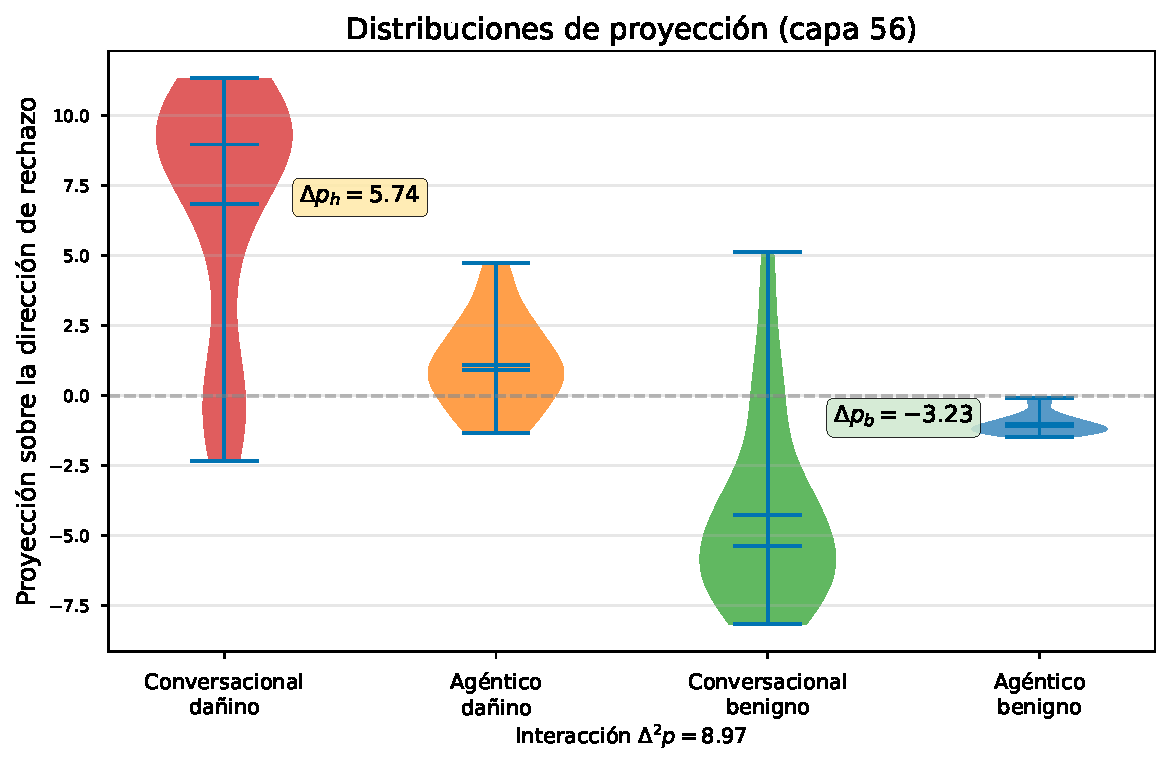
\includegraphics[width=0.86\linewidth]{es_distribuciones_capa56}
\caption{Distribuciones de proyección sobre la dirección de rechazo en la capa 56. Las instrucciones dañinas pierden proyección al pasar al formato agéntico y las benignas la ganan, de modo que ambas nubes convergen sobre el eje que las separaba. La interacción entre ambos desplazamientos es la cantidad específica del contenido dañino.}
\label{fig:distribuciones}
\end{figure}

Este patrón no es propio de una capa aislada. La interacción es positiva en las veinte capas evaluadas y crece de forma sostenida desde la capa 8 hasta la 56, como muestran la Tabla~\ref{tab:porcapa} y la Figura~\ref{fig:desplazamiento}. La regularidad es informativa por sí misma: un desplazamiento común a ambos brazos, atribuible a la longitud del estímulo o al mensaje de sistema, no tendría razón para acentuarse con la profundidad, mientras que un mecanismo que opera sobre la representación semántica de la petición sí la tiene. A partir de la capa 60 el desplazamiento y la interacción se reducen abruptamente en unidades crudas, comportamiento que se examina en el apartado siguiente.

\begin{figure}[htbp]
\centering
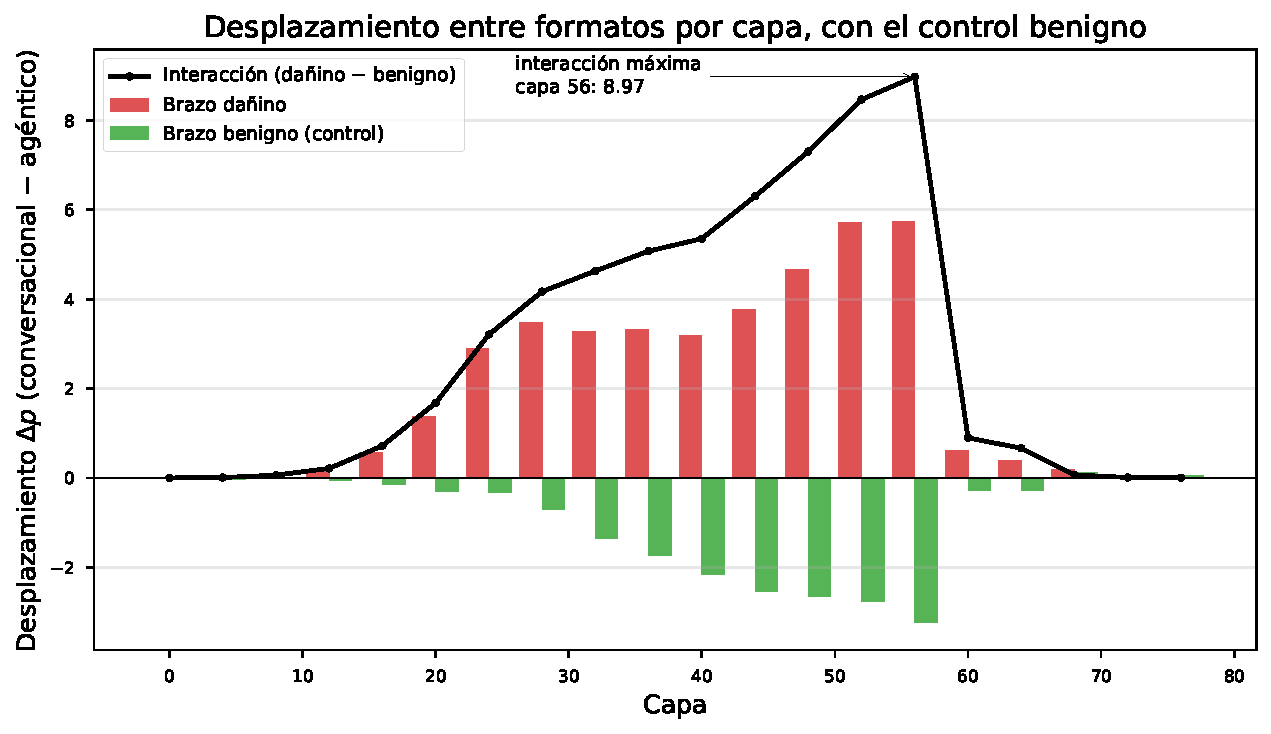
\includegraphics[width=0.95\linewidth]{es_desplazamiento_por_capa}
\caption{Desplazamiento entre formatos por capa, separado por brazo. El brazo dañino pierde proyección y el benigno la gana, de manera que la interacción, trazada como línea, excede en toda la red profunda al efecto principal.}
\label{fig:desplazamiento}
\end{figure}

\begin{table}[htbp]
\centering
\small
\setlength{\tabcolsep}{4pt}
\begin{tabular}{@{}rrrrccccc@{}}
\toprule
Capa & $\Delta p_{h}$ & $\Delta p_{b}$ & $\Delta^{2} p$ & $d_{\text{chat}}$ & $d_{\text{ag}}$ & AUROC$_{\text{chat}}$ & AUROC$_{\text{ag}}$ & Sonda (VC) \\
\midrule
0  & $-0{,}001$ & $-0{,}005$ & 0,004 & 1,51 & 1,36 & 0,853 & 0,840 & 0,724 \\
4  & $-0{,}012$ & $-0{,}025$ & 0,012 & 1,23 & 1,08 & 0,804 & 0,778 & 0,746 \\
8  & 0,049 & $-0{,}017$ & 0,066 & 2,04 & 1,83 & 0,924 & 0,899 & 0,815 \\
12 & 0,173 & $-0{,}043$ & 0,216 & 2,27 & 2,00 & 0,950 & 0,938 & 0,874 \\
16 & 0,575 & $-0{,}147$ & 0,722 & 2,93 & 1,90 & 0,984 & 0,950 & 0,946 \\
20 & 1,372 & $-0{,}308$ & 1,679 & 3,54 & 2,03 & 0,987 & 0,979 & 0,961 \\
24 & 2,892 & $-0{,}318$ & 3,209 & 3,44 & 1,67 & 0,978 & 0,976 & 0,958 \\
28 & 3,475 & $-0{,}695$ & 4,170 & 3,54 & 1,69 & 0,983 & 0,954 & 0,961 \\
32 & 3,276 & $-1{,}355$ & 4,631 & 3,48 & 1,69 & 0,981 & 0,929 & 0,956 \\
36 & 3,332 & $-1{,}741$ & 5,074 & 3,30 & 1,79 & 0,979 & 0,914 & 0,957 \\
40 & 3,188 & $-2{,}165$ & 5,353 & 3,27 & 2,02 & 0,979 & 0,922 & 0,953 \\
44 & 3,761 & $-2{,}540$ & 6,301 & 3,34 & 2,03 & 0,980 & 0,924 & 0,949 \\
48 & 4,662 & $-2{,}639$ & 7,301 & 3,33 & 2,03 & 0,980 & 0,928 & 0,948 \\
52 & \textbf{5,703} & $-2{,}759$ & \textbf{8,462} & 3,36 & 1,93 & 0,980 & 0,921 & 0,949 \\
56 & 5,739 & $-3{,}234$ & 8,973 & 2,93 & 1,83 & 0,969 & 0,905 & 0,947 \\
60 & 0,624 & $-0{,}277$ & 0,901 & 1,16 & 1,70 & 0,980 & 0,930 & 0,917 \\
64 & 0,395 & $-0{,}271$ & 0,667 & 0,39 & 1,70 & 0,945 & 0,904 & 0,818 \\
68 & 0,194 & 0,123 & 0,071 & 2,06 & 1,37 & 0,927 & 0,871 & 0,766 \\
72 & 0,062 & 0,047 & 0,014 & 1,25 & 0,98 & 0,811 & 0,763 & 0,722 \\
76 & 0,065 & 0,058 & 0,007 & 1,16 & 0,43 & 0,841 & 0,740 & 0,673 \\
\bottomrule
\end{tabular}
\caption{Desplazamiento entre formatos por capa en Llama-3.3-70B. $\Delta p_{h}$ y $\Delta p_{b}$ corresponden al brazo dañino y al benigno; $\Delta^{2} p$ es la interacción. Las columnas $d$ y AUROC expresan la separación entre clases dentro de cada formato en unidades estandarizadas y de rango, y se calculan sobre la muestra completa. En negrita, la capa de referencia.}
\label{tab:porcapa}
\end{table}

\subsection{Escala del efecto y localización en la red}

\justifying

Expresado en las tres unidades definidas en la formalización, el efecto de la capa 56 admite lecturas muy distintas en magnitud, y la discrepancia entre ellas constituye por sí misma un resultado. La separación entre clases cae de $11{,}097$ a $2{,}124$ en unidades crudas, esto es un $80{,}9\,\%$; en unidades estandarizadas cae de $d = 2{,}931$ a $d = 1{,}832$, un $37{,}5\,\%$. El factor de contracción de escala es $\kappa = 0{,}306$: la desviación estándar de las proyecciones en formato agéntico es menos de un tercio de la observada en el conversacional. Buena parte de la caída del $80{,}9\,\%$ es en consecuencia un cambio de unidades, y la cifra que corresponde al efecto es la estandarizada, con la cruda como su contraparte dependiente de escala.

Ese mismo argumento tiene una consecuencia sobre la localización del fenómeno. El criterio con que el procedimiento selecciona la capa es el desplazamiento en unidades crudas, y la norma del flujo residual crece con la profundidad, de modo que el criterio favorece a las capas tardías. El tamaño del efecto pareado no comparte esa dependencia, y su máximo dentro del bloque donde el desplazamiento tiene magnitud material cae en la capa 28 ($d_z = 3{,}14$) y no en la 56 ($d_z = 1{,}63$). La Figura~\ref{fig:crudo} muestra ambos criterios sobre el mismo eje.

\begin{figure}[htbp]
\centering
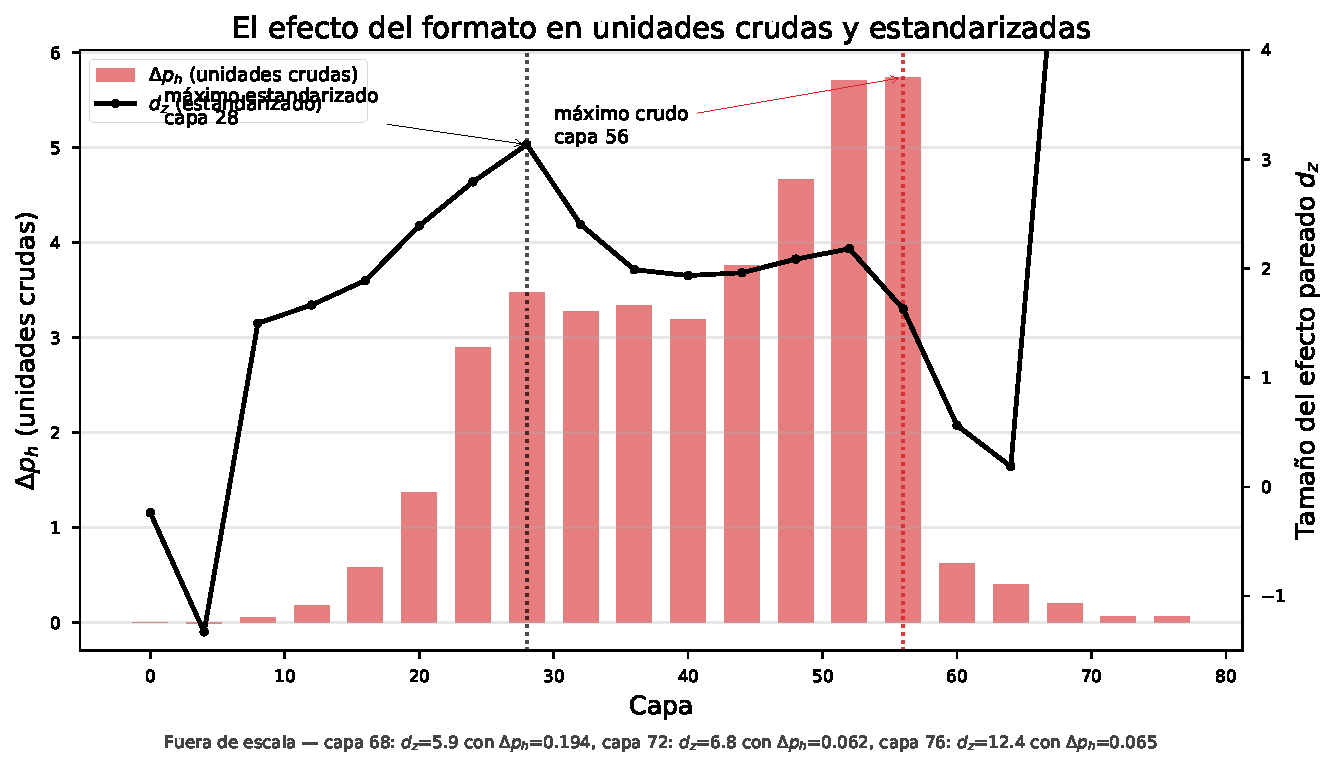
\includegraphics[width=0.95\linewidth]{es_crudo_vs_estandarizado}
\caption{El efecto del formato medido en unidades crudas y estandarizadas. El desplazamiento crudo alcanza su máximo en la capa 56, arrastrado por el crecimiento de la norma del flujo residual con la profundidad; el tamaño del efecto pareado lo alcanza en la capa 28. En las tres capas finales el desplazamiento es diminuto pero casi idéntico en los 42 pares, de modo que allí $d_z$ describe consistencia y no magnitud.}
\label{fig:crudo}
\end{figure}

La capa 28 concentra además el resto de los indicadores del fenómeno, como recoge la Tabla~\ref{tab:localizacion}: es la capa donde la sonda validada alcanza su máximo ($0{,}961$), donde el sesgo de estimación es menor ($1{,}7\,\%$), donde la dirección agéntica es más ortogonal a la conversacional ($\cos = 0{,}031$) y donde el monitor evaluado fuera de fold obtiene su mejor desempeño ($F_1 = 0{,}909$). Cuatro criterios independientes entre sí, y ninguno dependiente de la escala de las proyecciones, coinciden en la misma región de la red.

La caída abrupta del desplazamiento a partir de la capa 60 se explica en los mismos términos. En esa región las distribuciones de proyección se vuelven marcadamente asimétricas: en la capa 64 la proyección media de las instrucciones dañinas en formato conversacional es $0{,}38$ con desviación estándar de $2{,}11$ y un máximo de $13{,}74$. Unas pocas instrucciones de proyección muy elevada deprimen el $d$ de Cohen, cuyo denominador recoge la dispersión inducida por las colas, mientras que el AUROC, basado en rangos, permanece en $0{,}945$. La divergencia entre ambas medidas en ese tramo informa que la separación persiste en el ordenamiento aunque no en la distancia estandarizada, y desaconseja leer las capas finales con las mismas herramientas que el bloque profundo-medio.

\begin{table}[htbp]
\centering
\small
\setlength{\tabcolsep}{5pt}
\begin{tabular}{@{}rrccrccc@{}}
\toprule
Capa & $\Delta p_{h}$ & $d_z$ & IC 95\,\% (BCa) & Sesgo & Sonda (VC) & $\cos(\bm{w}_{\text{ag}},\hat{\bm{r}})$ & $F_1$ monitor \\
\midrule
16 & 0,575 & 1,89 & [0,477; 0,669] & 12,1\,\% & 0,946 & 0,333 & 0,831 \\
20 & 1,372 & 2,39 & [1,198; 1,562] & 5,5\,\% & 0,961 & 0,274 & 0,854 \\
24 & 2,892 & 2,79 & [2,546; 3,170] & 2,4\,\% & 0,958 & 0,131 & 0,864 \\
28 & 3,475 & \textbf{3,14} & [3,105; 3,756] & \textbf{1,7\,\%} & \textbf{0,961} & \textbf{0,031} & \textbf{0,909} \\
32 & 3,276 & 2,40 & [2,839; 3,643] & 1,4\,\% & 0,956 & 0,060 & 0,837 \\
40 & 3,188 & 1,94 & [2,637; 3,646] & 1,6\,\% & 0,953 & 0,045 & 0,851 \\
48 & 4,662 & 2,09 & [3,946; 5,255] & 2,2\,\% & 0,948 & 0,048 & 0,851 \\
52 & 5,703 & 2,18 & [4,829; 6,394] & 2,4\,\% & 0,949 & 0,047 & 0,854 \\
56 & 5,739 & 1,63 & [4,625; 6,704] & 4,4\,\% & 0,947 & 0,051 & 0,837 \\
60 & 0,624 & 0,56 & [0,434; 1,301] & 108\,\% & 0,917 & 0,290 & 0,821 \\
64 & 0,395 & 0,19 & [0,065; 1,711] & 408\,\% & 0,818 & 0,149 & 0,723 \\
\bottomrule
\end{tabular}
\caption{Localización del fenómeno según criterios independientes de la escala. La columna de sesgo expresa la diferencia entre el desplazamiento estimado con la dirección ajustada sobre toda la muestra y el estimado con validación cruzada, como porcentaje de este último. En negrita, los valores óptimos, que coinciden en la capa 28.}
\label{tab:localizacion}
\end{table}

\subsection{Estabilidad de la estimación y análisis de sensibilidad}

\justifying

La corrección por circularidad verifica que el desplazamiento no sea un artefacto de estimar la dirección sobre las mismas activaciones que después se proyectan. En la capa 56, al recalcular la dirección fuera de muestra, $\Delta p_{h}$ desciende de $5{,}739$ a $5{,}497$, lo que sitúa el sesgo en $0{,}242$, un $4{,}4\,\%$ del valor corregido, con intervalo $[4{,}446;\ 6{,}514]$ y $d_z = 1{,}591$.

El comportamiento del sesgo a lo largo de la red, recogido en la Figura~\ref{fig:deteccion} y en la Tabla~\ref{tab:localizacion}, aporta un criterio adicional de credibilidad. Entre las capas 24 y 56 el sesgo se mantiene entre el $1{,}4\,\%$ y el $4{,}4\,\%$ del efecto, mientras que en las capas 60 y 64 alcanza el $108\,\%$ y el $408\,\%$, hasta el punto de que en la capa 64 la estimación corregida invierte el signo ($-0{,}128$ frente a $+0{,}395$). La región donde el efecto es sustantivo coincide con la región donde la estimación de la dirección es estable, y la región donde la estimación es frágil es también aquella donde el efecto aparente carece de magnitud.

El análisis de sensibilidad se realiza sobre la capa 52, seleccionada por división de muestra y por tanto ajena a los datos con que se realiza la inferencia. En ella $\Delta p_{h} = 5{,}703$, con intervalo BCa de $[4{,}829;\ 6{,}394]$, $d_z = 2{,}18$ y 39 de 42 pares decreciendo; la corrección por circularidad la reduce a $5{,}570$, un sesgo del $2{,}4\,\%$. El control benigno mantiene el signo y la magnitud del hallazgo: $\Delta p_{b} = -2{,}759$ y una interacción de $8{,}462$, con fracción común de $-48{,}4\,\%$. En unidades invariantes a la escala, la separación estandarizada cae de $3{,}355$ a $1{,}928$, un $42{,}5\,\%$, con contracción de escala $\kappa = 0{,}341$. La conclusión del análisis de sensibilidad es que ninguna afirmación de este capítulo depende de la capa que el procedimiento seleccionó: en la capa elegida sin contaminación por comparación múltiple el efecto conserva signo, significancia, especificidad y orden de magnitud, y varía únicamente la cifra cruda, que es la dependiente de escala.

\begin{figure}[htbp]
\centering
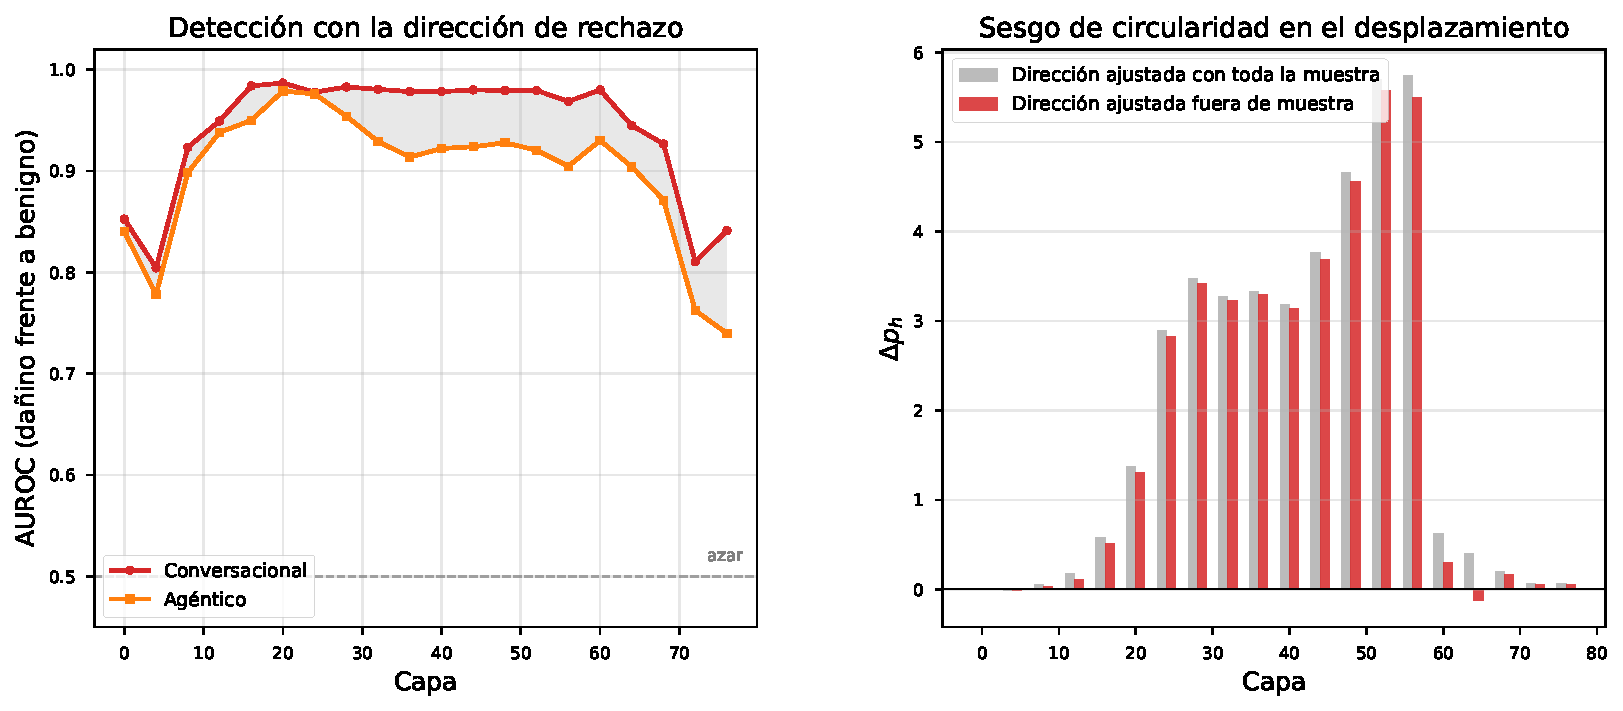
\includegraphics[width=\linewidth]{es_deteccion_y_circularidad}
\caption{Izquierda: capacidad de discriminación de la dirección de rechazo en cada formato, por capa; el área sombreada es el gap de detección. Derecha: desplazamiento estimado con la dirección ajustada sobre toda la muestra y con la dirección ajustada fuera de muestra. El sesgo de estimación es pequeño en el bloque donde el efecto es sustantivo y desproporcionado en las capas 60 a 64, donde el efecto aparente carece de magnitud.}
\label{fig:deteccion}
\end{figure}

\subsection{El gap de detección, una cantidad distinta}

\justifying

Junto al gap de proyección, el análisis reporta una segunda diferencia entre formatos que conviene no confundir con aquella. El gap de detección es la diferencia entre el AUROC del formato conversacional y el del agéntico. Como el AUROC es la probabilidad de que una instrucción dañina proyecte más que una benigna tomadas al azar, su diferencia entre formatos cuenta la proporción de comparaciones dañino--benigno que el formato conversacional ordena correctamente y el agéntico deja de ordenar correctamente: es decir, los casos que el modelo sitúa por encima del umbral de peligrosidad cuando conversa y por debajo cuando dispone de herramientas.

En la capa de referencia el AUROC pasa de $0{,}980$ a $0{,}921$, un gap de $0{,}059$. Entre los 42 pares dañinos y los 42 benignos existen 1.764 comparaciones posibles; el gap corresponde por tanto a un saldo neto de unas 104 comparaciones que el formato conversacional ordena correctamente y el agéntico no. Se trata de un saldo, y no de un recuento bruto, porque algunas comparaciones pueden ordenarse mejor bajo el formato agéntico y el gap ya las descuenta. En la capa 56 asciende a $0{,}064$, equivalente a unas 113 comparaciones. La brecha no es uniforme a lo largo de la red: es de $0{,}008$ en la capa 20, alcanza $0{,}029$ en la 28, $0{,}052$ en la 32 y $0{,}064$ en la 56. En las capas iniciales la dirección conserva prácticamente intacta su capacidad discriminativa al cambiar de formato, y la degradación se concentra en el bloque profundo. El panel izquierdo de la Figura~\ref{fig:deteccion} muestra que la curva agéntica discurre por debajo de la conversacional en todo el tramo posterior a la capa 24, sin aproximarse en ningún punto al azar.

Las dos cantidades responden a preguntas distintas y por eso arrojan magnitudes distintas. El gap de proyección mide la intensidad con que la representación de rechazo responde ante una petición peligrosa, y cae un $37{,}5\,\%$ en unidades estandarizadas. El gap de detección mide si esa respuesta sigue bastando para separar lo dañino de lo inocuo, y cae un $6{,}4\,\%$. Que la segunda cifra sea mucho menor que la primera no las contradice: el AUROC es una medida de ordenamiento y se satura, de modo que una pérdida considerable de margen puede producirse sin que muchas comparaciones lleguen a cruzar el umbral. El hallazgo central de este trabajo es el gap de proyección junto con su especificidad respecto del brazo benigno; el gap de detección lo acompaña como indicación de cuánto de esa pérdida de margen se traduce, con este corpus, en una pérdida efectiva de discriminación.

Los valores de AUROC por formato de las Tablas~\ref{tab:porcapa} y \ref{tab:escala} se calculan sobre la muestra completa. La magnitud de la inflación asociada puede acotarse para el brazo conversacional con la validación cruzada de la sonda, que reajusta la dirección dentro de cada partición: el AUROC de la dirección fuera de fold es $0{,}977$ en la capa 52 y $0{,}978$ en la 28, frente a $0{,}980$ y $0{,}983$ sobre la muestra completa, de modo que la inflación es del orden de $0{,}005$, dos órdenes de magnitud menor que la observada en la sonda entrenada. La diferencia entre ambos casos tiene explicación geométrica: la dirección de diferencia de medias está determinada por dos promedios, mientras que la sonda ajusta un hiperplano completo y, con 84 puntos en 8192 dimensiones, dispone de holgura para separar cualquier etiquetado.

\begin{table}[htbp]
\centering
\small
\begin{tabular}{@{}lccc@{}}
\toprule
Medida (capa 56) & Conversacional & Agéntico & Pérdida \\
\midrule
Separación (unidades crudas) & 11,097 & 2,124 & 80,9\,\% \\
Desviación estándar agrupada & 3,786 & 1,160 & --- \\
Separación estandarizada ($d$) & 2,931 & 1,832 & 37,5\,\% \\
AUROC & 0,969 & 0,905 & 6,4\,\% \\
\midrule
\multicolumn{4}{@{}l}{Factor de contracción de escala $\kappa = 0{,}306$} \\
\bottomrule
\end{tabular}
\caption{El mismo efecto expresado en tres unidades. La discrepancia entre la pérdida cruda y la estandarizada mide qué parte del desplazamiento corresponde a un cambio de escala; la fila del AUROC corresponde al gap de detección, que es una cantidad distinta del gap de proyección.}
\label{tab:escala}
\end{table}

\subsection{Comportamiento según el grado de explicitud}

\justifying

El análisis por estrato responde al cuarto objetivo específico, y su lectura debe ser prudente: los tres estratos cuentan con 18, 14 y 10 pares respectivamente, de modo que las cifras que siguen describen un patrón exploratorio y no una relación establecida.

Medido por el gap de proyección, el desplazamiento decrece al disminuir la explicitud del daño: $6{,}675$ en el estrato explícito, $6{,}360$ en el contextual y $3{,}186$ en el de apariencia legítima. Los intervalos de confianza, sin embargo, no sostienen esa ordenación. Los de los estratos explícito y contextual se solapan casi por completo ($[5{,}212;\ 7{,}884]$ y $[4{,}714;\ 7{,}834]$), de manera que el orden entre ambos no está respaldado por los datos. El estrato de apariencia legítima presenta el desplazamiento más bajo y su intervalo, $[0{,}927;\ 5{,}506]$, se solapa con los otros dos en su extremo superior, con una significancia marginal ($p = 0{,}045$) sobre diez pares. Lo que los datos sostienen, en consecuencia, es que el efecto está presente en los tres estratos; la ordenación entre ellos requiere un corpus mayor para ser afirmada.

Medido por el gap de detección la tendencia aparente se invierte, lo que refuerza la conveniencia de tratar ambos gaps como cantidades separadas. La pérdida de AUROC es de $0{,}065$ en el estrato explícito ($0{,}981 \rightarrow 0{,}917$), $0{,}051$ en el contextual y $0{,}050$ en el de apariencia legítima, y la pérdida de separación estandarizada alcanza su valor mayor en el estrato contextual ($47{,}0\,\%$) y el menor en el de apariencia legítima ($6{,}4\,\%$). Una lectura compatible con estas cifras, y que el diseño no permite confirmar con este número de casos, es que el formato agéntico erosiona sobre todo el margen allí donde era más amplio, mientras que en las instrucciones encubiertas el margen ya era estrecho en el formato conversacional y se degrada poco.

Con independencia de la ordenación, el resultado que sí se sostiene es que la detección se mantiene por encima de $0{,}88$ en los tres estratos bajo el formato agéntico: la dirección conserva poder discriminativo incluso ante intención encubierta, con un margen sensiblemente menor que en el formato conversacional. La Tabla~\ref{tab:estratos} recoge las cifras.

\begin{table}[htbp]
\centering
\small
\setlength{\tabcolsep}{5pt}
\begin{tabular}{@{}lcrcccc@{}}
\toprule
Estrato & $n$ & $\Delta p_{h}$ & IC 95\,\% & AUROC$_{\text{chat}}$ & AUROC$_{\text{ag}}$ & Pérdida en $d$ \\
\midrule
Explícito & 18 & 6,675 & [5,212; 7,884] & 0,981 & 0,917 & 38,1\,\% \\
Contextual & 14 & 6,360 & [4,714; 7,834] & 0,980 & 0,929 & 47,0\,\% \\
Apariencia legítima & 10 & 3,186 & [0,927; 5,506] & 0,930 & 0,880 & 6,4\,\% \\
\bottomrule
\end{tabular}
\caption{Gap de proyección y gap de detección por grado de explicitud de la intención dañina (capa 56). Los intervalos se solapan entre estratos, de modo que las cifras describen un patrón exploratorio y no una ordenación establecida.}
\label{tab:estratos}
\end{table}

\subsection{Rotación de la dirección y viabilidad del monitoreo}

\justifying

El desplazamiento de la proyección viene acompañado de un cambio de eje. Al estimar por diferencia de medias una dirección propia del formato agéntico, denotada $\bm{w}_{\text{ag}}$, y compararla con la dirección de rechazo conversacional, el coseno entre ambas cae desde aproximadamente $0{,}46$ en las capas iniciales hasta $0{,}031$ en la capa 28, no supera $0{,}06$ en todo el bloque profundo-medio y vuelve a ascender hacia la salida. En las capas donde el efecto de formato es más intenso, la dirección que separa lo dañino de lo benigno en contexto agéntico es prácticamente ortogonal a la dirección de rechazo conversacional.

La estimación fuera de fold del coseno arroja $0{,}047 \pm 0{,}009$ en la capa 56, prácticamente idéntica al valor sobre la muestra completa. La fiabilidad de la estimación de $\bm{w}_{\text{ag}}$, medida sobre mitades disjuntas de la muestra, es baja ($0{,}188$), lo que implica que el coseno observado está atenuado por ruido de medición; corrigiendo por atenuación, el valor verdadero rondaría $0{,}11$, que sigue correspondiendo a un ángulo próximo a la ortogonalidad. La conclusión sobre la rotación no depende, por tanto, de que el ruido esté aplastando una correlación real, aunque el margen de error es amplio.

La información permanece presente y linealmente separable en el formato agéntico. La dirección agéntica alcanza un AUROC fuera de fold de $0{,}917 \pm 0{,}055$ en la capa 56 y de $0{,}951 \pm 0{,}079$ en la capa 28, frente al valor de $1{,}000$ sobre la muestra completa que la geometría del problema garantiza de antemano. Un monitor construido sobre esa dirección, con umbral calibrado fuera de fold, obtiene en la capa 28 una puntuación $F_1$ de $0{,}909$, con precisión $0{,}870$, exhaustividad $0{,}952$ y tasa de falsos positivos de $0{,}143$; en la capa 52 el desempeño es de $F_1 = 0{,}854$ con tasa de falsos positivos de $0{,}214$. El panel derecho de la Figura~\ref{fig:rotacion} muestra que el desempeño del monitor sigue a lo largo de la red la misma forma que la accesibilidad lineal de la sonda, con un máximo amplio en el bloque intermedio, y que la tasa de falsos positivos describe la trayectoria inversa. Una tasa de entre el catorce y el veintiuno por ciento es elevada para un despliegue real, de modo que la exploración establece la viabilidad del enfoque y no la de un sistema en condiciones de producción.

\begin{figure}[htbp]
\centering
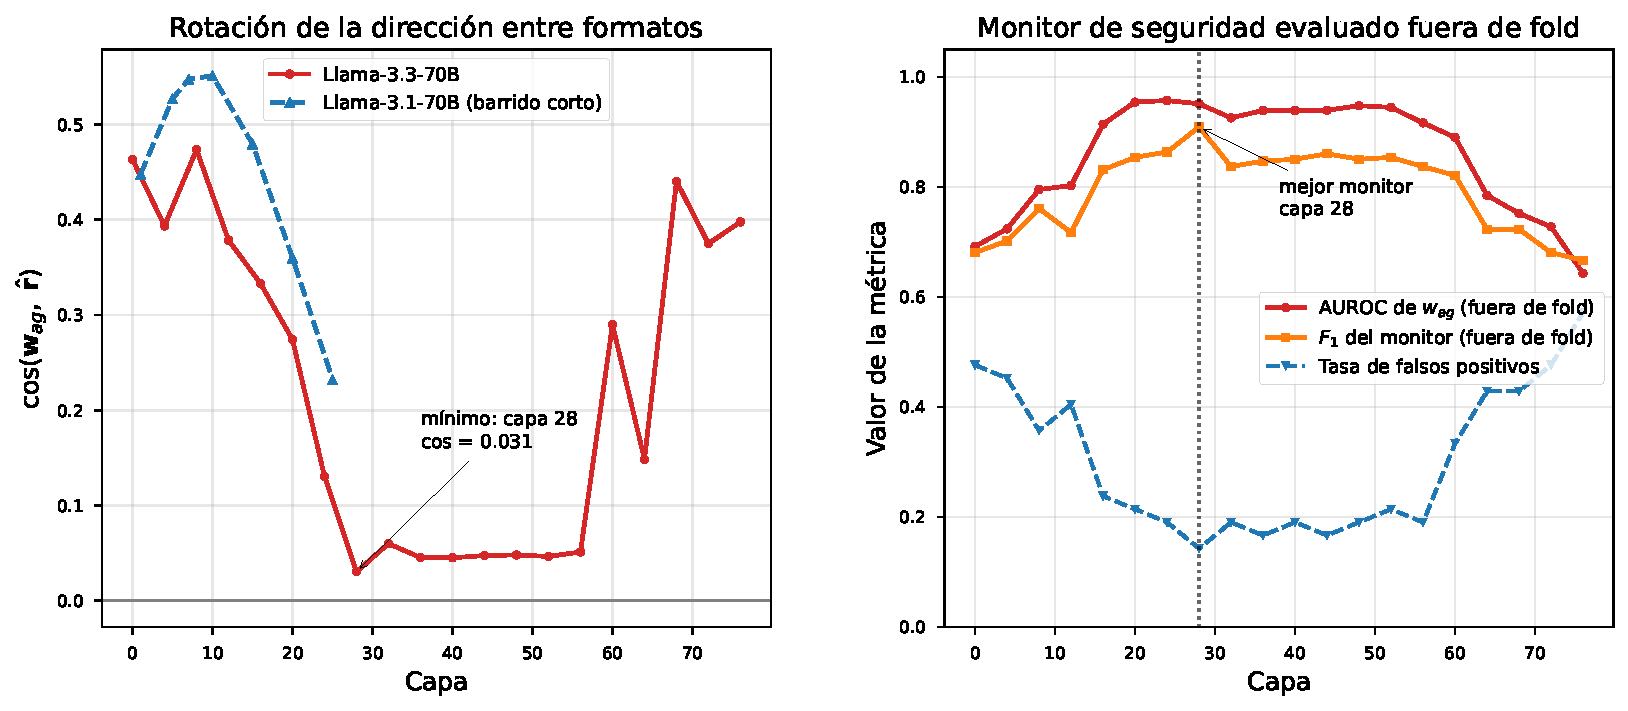
\includegraphics[width=\linewidth]{es_rotacion_y_monitor}
\caption{Izquierda: coseno entre la dirección estimada en formato agéntico y la dirección de rechazo conversacional, en los dos puntos de control. La corrida corta sobre Llama-3.1-70B recorre el mismo descenso y se detiene antes del mínimo. Derecha: desempeño del monitor construido sobre la dirección agéntica, con dirección y umbral estimados fuera de fold.}
\label{fig:rotacion}
\end{figure}

Estos resultados delinean un modo de fallo preciso para el monitoreo. El modelo no deja de codificar la peligrosidad de una instrucción cuando opera como agente: la codifica sobre un eje distinto. Un monitor construido sobre representaciones conversacionales, que es la práctica que la caracterización disponible en la literatura sugiere \parencite{arditi2024}, mediría en una dirección casi ortogonal a aquella en la que la información reside.

\subsection{Replicación entre puntos de control}

\justifying

La comparación entre las dos corridas, resumida en la Tabla~\ref{tab:comparacion}, replica el hallazgo en su signo y en su estructura. En la única capa que ambas comparten, la 20, el gap de proyección es de $0{,}684$ en Llama-3.1-70B y de $1{,}372$ en Llama-3.3-70B; en ambos casos la totalidad de los 42 pares decrece y ambos intervalos excluyen el cero. La rotación de la dirección también se replica: el coseno con la dirección conversacional desciende en Llama-3.1-70B de $0{,}551$ en la capa 10 a $0{,}233$ en la capa 25, y en Llama-3.3-70B recorre el mismo descenso en el mismo tramo, de $0{,}474$ en la capa 8 a $0{,}131$ en la 24, para continuar hasta $0{,}031$ en la 28. Como muestra el panel izquierdo de la Figura~\ref{fig:rotacion}, las dos curvas describen la misma trayectoria y la corrida corta se interrumpe justo antes del mínimo.

La comparación advierte además sobre un riesgo metodológico. La corrida sobre Llama-3.1-70B se detuvo en la capa 25, y dentro de esa ventana el desplazamiento venía creciendo de forma sostenida ($0{,}054$ en la capa 10, $0{,}238$ en la 15, $0{,}684$ en la 20) con un leve descenso en la capa 25 que aparentaba ser un máximo. El barrido completo muestra que no lo era: el efecto continúa creciendo hasta $5{,}70$ en la capa 52. La conclusión que se derivaba de la corrida corta, según la cual el desplazamiento disminuye pero la detección se preserva, era un artefacto de la ventana observada, pues en la capa 20 el gap de detección es de apenas $0{,}008$ en ambas corridas. En las capas profundas, en cambio, la detección sí se degrada, de $0{,}980$ a $0{,}921$ en la capa de referencia. Las dos corridas no se contradicen: la primera no alcanzó la región donde reside el efecto.

El mismo desplazamiento de ventana explica la diferencia en el análisis por estrato. En la capa 20 de Llama-3.1-70B los tres estratos presentan desplazamientos equivalentes ($0{,}720$ explícito, $0{,}701$ contextual, $0{,}597$ apariencia legítima), sin la separación entre el estrato de apariencia legítima y los otros dos que se observa en la capa 56 de la corrida completa.

\begin{table}[htbp]
\centering
\small
\begin{tabular}{@{}lcc@{}}
\toprule
 & Llama-3.1-70B & Llama-3.3-70B \\
\midrule
Capas evaluadas & 7 (1 a 25) & 20 (0 a 76) \\
Capa reportada & 20 & 56 \\
$\Delta p_{h}$ en la capa reportada & 0,684 & 5,739 \\
IC 95\,\% (BCa) & [0,580; 0,782] & [4,618; 6,725] \\
Pares que decrecen & 42/42 & 36/42 \\
$d_z$ pareada & 2,080 & 1,629 \\
$\Delta p_{h}$ en la capa 20 & 0,684 & 1,372 \\
Gap de detección en la capa 20 & 0,001 & 0,008 \\
$\cos(\bm{w}_{\text{ag}}, \hat{\bm{r}})$ en la capa 20 & 0,360 & 0,274 \\
Capas con IC que excluye el cero & 6/7 & 19/20 \\
AUROC de la sonda & 1,000 (división única) & 0,961 $\pm$ 0,040 (10$\times$5 VC) \\
\bottomrule
\end{tabular}
\caption{Comparación entre los dos puntos de control evaluados. La diferencia principal entre ambas columnas no proviene del modelo sino de la extensión del barrido de capas.}
\label{tab:comparacion}
\end{table}

\subsection{Síntesis y alcance de validez}

\justifying

El resultado central es el gap de proyección sobre la dirección de rechazo. Una misma instrucción dañina, con texto idéntico, proyecta $5{,}74$ unidades menos sobre esa dirección cuando el modelo dispone de herramientas (IC 95\,\% $[4{,}62;\ 6{,}73]$; 36 de 42 pares; $5{,}70$ con IC $[4{,}83;\ 6{,}39]$ en la capa de referencia del análisis de sensibilidad), y el efecto sobrevive a la corrección por circularidad con un sesgo de entre el $2{,}4\,\%$ y el $4{,}4\,\%$. Ese desplazamiento es específico del contenido dañino: el brazo benigno se mueve en sentido contrario, la interacción alcanza $+8{,}97$ con $d = 2{,}67$, y queda descartado que se trate de una traslación común a toda representación. En unidades invariantes a la escala la respuesta de la representación de rechazo se reduce en un $37{,}5\,\%$, mientras la desviación estándar de las proyecciones se contrae a menos de un tercio.

Dos resultados acompañan al anterior. El primero es que la información no desaparece sino que se reorganiza sobre un eje distinto, casi ortogonal al conversacional en las capas donde el efecto es más intenso, y sigue siendo recuperable por una dirección estimada dentro del propio formato agéntico ($F_1 = 0{,}909$ fuera de fold en la capa 28). El segundo es que el gap de detección, cantidad distinta de la anterior, es de $0{,}059$ en la capa de referencia: en términos netos, alrededor de 104 de las 1.764 comparaciones dañino--benigno que el formato conversacional ordena correctamente dejan de ordenarse correctamente en el agéntico. La detección se degrada, por tanto, mucho menos que la intensidad de la respuesta, lo que sitúa el fenómeno como una pérdida de margen y no como un colapso de la discriminación.

En cuanto al alcance de estas conclusiones, cinco condiciones lo delimitan. La primera es que las afirmaciones se refieren al vínculo entre el formato y la representación, no al vínculo entre la representación y el comportamiento; la etapa de intervención, que es la que permitiría cerrar el segundo, no se reporta en esta corrida por un defecto de implementación en la construcción del estímulo de la rutina de generación, cuya corrección y repetición forman parte del trabajo previsto. La segunda es el tamaño del corpus: 42 pares determinan la precisión de todas las estimaciones, y son la razón por la que el intervalo de la sonda alcanza el techo del AUROC y por la que la ordenación entre estratos solo puede presentarse como patrón exploratorio. La tercera es que las dos corridas pertenecen a la misma familia y comparten arquitectura, de modo que lo replicado es un punto de control y no una familia distinta. La cuarta es la fiabilidad de la estimación de la dirección agéntica, de $0{,}188$, que obliga a leer las cifras del coseno con el margen que la corrección por atenuación hace explícito. La quinta es que los valores de AUROC por formato se calculan sobre la muestra completa, con una inflación acotada en el brazo conversacional del orden de $0{,}005$.

% ==================== REFERENCIAS ====================
\newpage
\section*{Referencias}
\addcontentsline{toc}{section}{Referencias}

\begin{thebibliography}{99}
\setlength{\itemsep}{0.6em}
\bibitem[Andriushchenko et al.(2024)]{andriushchenko2024}%
Andriushchenko, M., Souly, A., Dziemian, M., Duenas, D., Lin, M., Wang, J., \ldots\ Davies, X. (2024). \textit{AgentHarm: A benchmark for measuring harmfulness of LLM agents}. arXiv:2410.09024. \url{https://arxiv.org/abs/2410.09024}

\bibitem[Alain \& Bengio(2017)]{alain2017}
Alain, G., \& Bengio, Y. (2017). \textit{Understanding intermediate layers using linear classifier probes}. International Conference on Learning Representations (ICLR), Workshop Track. arXiv:1610.01644. \url{https://arxiv.org/abs/1610.01644}

\bibitem[Arditi et al.(2024)]{arditi2024}
Arditi, A., Obeso, O., Syed, A., Paleka, D., Panickssery, N., Gurnee, W., \& Nanda, N. (2024). \textit{Refusal in language models is mediated by a single direction}. Advances in Neural Information Processing Systems (NeurIPS 2024). arXiv:2406.11717. \url{https://arxiv.org/abs/2406.11717}

\bibitem[Bai et al.(2022)]{bai2022}
Bai, Y., Kadavath, S., Kundu, S., Askell, A., Kernion, J., Jones, A., \ldots\ Kaplan, J. (2022). \textit{Constitutional AI: Harmlessness from AI feedback}. arXiv:2212.08073. \url{https://arxiv.org/abs/2212.08073}

\bibitem[Dur\'an et al.(2025)]{ilia2025}
Dur\'an, R., Moreno, A., Adasme, S., Rovira, S., Jord\'an, V., \& Poveda, L. (Coords.). (2025). \textit{\'Indice Latinoamericano de Inteligencia Artificial (ILIA) 2025}. Documentos de Proyectos (LC/TS.2025/68). Comisi\'on Econ\'omica para Am\'erica Latina y el Caribe (CEPAL) y Centro Nacional de Inteligencia Artificial (CENIA). \url{https://www.cepal.org/es/publicaciones/82514-indice-latinoamericano-inteligencia-artificial-ilia-2025}

\bibitem[Gravitee(2026)]{gravitee2026}
Gravitee. (2026). \textit{State of AI agent security 2026 report: When adoption outpaces control}. \url{https://www.gravitee.io/blog/state-of-ai-agent-security-2026-report-when-adoption-outpaces-control}

\bibitem[Greenblatt et al.(2024)]{greenblatt2024}
Greenblatt, R., Denison, C., Wright, B., Roger, F., MacDiarmid, M., Marks, S., \ldots\ Hubinger, E. (2024). \textit{Alignment faking in large language models}. arXiv:2412.14093. \url{https://arxiv.org/abs/2412.14093}

\bibitem[Lermen et al.(2024)]{lermen2024}
Lermen, S., Dziemian, M., \& Pimpale, G. (2024). \textit{Applying refusal-vector ablation to Llama 3.1 70B agents}. arXiv:2410.10871. \url{https://arxiv.org/abs/2410.10871}

\bibitem[miniOrange(2026)]{miniorange2026}
miniOrange. (2026). \textit{AI agent security risks: What enterprises need to know in 2026}. \url{https://www.miniorange.com/blog/ai-agent-security-risks/}

\bibitem[Olah et al.(2020)]{olah2020}
Olah, C., Cammarata, N., Schubert, L., Goh, G., Petrov, M., \& Carter, S. (2020). \textit{Zoom In: An Introduction to Circuits}. Distill, 5(3). \url{https://distill.pub/2020/circuits/zoom-in/} \mbox{https://doi.org/10.23915/distill.00024.001}

\bibitem[Ouyang et al.(2022)]{ouyang2022}
Ouyang, L., Wu, J., Jiang, X., Almeida, D., Wainwright, C., Mishkin, P., \ldots\ Lowe, R. (2022). \textit{Training language models to follow instructions with human feedback}. Advances in Neural Information Processing Systems (NeurIPS 2022). arXiv:2203.02155. \url{https://arxiv.org/abs/2203.02155}

\bibitem[Park et al.(2024)]{park2024}
Park, K., Choe, Y. J., \& Veitch, V. (2024). \textit{The linear representation hypothesis and the geometry of large language models}. International Conference on Machine Learning (ICML). arXiv:2311.03658. \url{https://arxiv.org/abs/2311.03658}

\bibitem[Pinto(2026)]{pinto2026}
Pinto, L. (2026). \textit{Present but rescaled: Chat-to-agent transfer of additive activation steering}. arXiv:2607.09156. \url{https://arxiv.org/abs/2607.09156}

\bibitem[Templeton et al.(2024)]{templeton2024}
Templeton, A., Conerly, T., Marcus, J., Lindsey, J., Bricken, T., Chen, B., \ldots\ Henighan, T. (2024). \textit{Scaling monosemanticity: Extracting interpretable features from Claude 3 Sonnet}. Transformer Circuits. \url{https://transformer-circuits.pub/2024/scaling-monosemanticity/}

\bibitem[Zhong et al.(2026)]{zhong2026}
Zhong, V., et al. (2026). \textit{Refusal lives downstream of persona in chat models}. arXiv:2606.26161. \url{https://arxiv.org/abs/2606.26161}

\bibitem[Zou et al.(2023)]{zou2023}
Zou, A., Phan, L., Chen, S., Campbell, J., Guo, P., Ren, R., \ldots\ Hendrycks, D. (2023). \textit{Representation engineering: A top-down approach to AI transparency}. arXiv:2310.01405. \url{https://arxiv.org/abs/2310.01405}

\end{thebibliography}

\end{document}
